\documentclass[runningheads]{llncs}

% ---------------------------------------------------------------
% Include basic ECCV package
 
% TODO REVIEW: Insert your submission number below by replacing '*****'
% TODO FINAL: Comment out the following line for the camera-ready version
\usepackage[review,year=2024,ID=4126]{eccv}
% TODO FINAL: Un-comment the following line for the camera-ready version
%\usepackage{eccv}

% OPTIONAL: Un-comment the following line for a version which is easier to read
% on small portrait-orientation screens (e.g., mobile phones, or beside other windows)
%\usepackage[mobile]{eccv}


% Import additional packages in the preamble file, before hyperref
%
% --- inline annotations
%
% \usepackage[dvipsnames]{xcolor}
% \newcommand{\red}[1]{{\color{red}#1}}
% \newcommand{\todo}[1]{{\color{red}#1}}
% \newcommand{\TODO}[1]{\textbf{\color{red}[TODO: #1]}}
% --- disable by uncommenting  
% \renewcommand{\TODO}[1]{}
% \renewcommand{\todo}[1]{#1}

\usepackage{microtype,nicefrac,amsfonts,times,epsfig,graphicx,amsmath,amssymb,booktabs,comment,tabulary,multirow,xspace,rotating,url,makecell,soul,setspace,pifont,makebox,threeparttable,tablefootnote}
\usepackage[font=small]{caption}
\usepackage[capbesideposition=outside,capbesidesep=quad]{floatrow}

\usepackage{colortbl}
\usepackage{enumitem}
\usepackage{xcolor}
% \usepackage[utf8]{inputenc} % allow utf-8 input
\usepackage[T1]{fontenc}    % use 8-bit T1 fonts
\usepackage{wrapfig}


% ---------------------------------------------------------------
% Other packages

% Commonly used abbreviations (\eg, \ie, \etc, \cf, \etal, etc.)
\usepackage{eccvabbrv}

% Include other packages here, before hyperref.
\usepackage{graphicx}
\usepackage{booktabs}

% The "axessiblity" package can be found at: https://ctan.org/pkg/axessibility?lang=en
\usepackage[accsupp]{axessibility}  % Improves PDF readability for those with disabilities.


% ---------------------------------------------------------------
% Hyperref package

% It is strongly recommended to use hyperref, especially for the review version.
% Please disable hyperref *only* if you encounter grave issues.
% hyperref with option pagebackref eases the reviewers' job, but should be disabled for the final version.
%
% If you comment hyperref and then uncomment it, you should delete
% main.aux before re-running LaTeX.
% (Or just hit 'q' on the first LaTeX run, let it finish, and you
%  should be clear).

% TODO FINAL: Comment out the following line for the camera-ready version
\usepackage[pagebackref,breaklinks,colorlinks,citecolor=eccvblue]{hyperref}
% TODO FINAL: Un-comment the following line for the camera-ready version
%\usepackage{hyperref}

% Support for ORCID icon
\usepackage{orcidlink}


\definecolor{mygray}{rgb}{0.5, 0.5, 0.5}
\definecolor{fpn}{HTML}{04d45e}
\definecolor{ss}{HTML}{ff8408}

% comments
\newcommand{\cs}[1]{\textcolor{magenta}{CS: #1}}
\newcommand{\kien}[1]{\textcolor{blue}{DK: #1}}
\newcommand{\mo}[1]{\textcolor{red}{MO: #1}}

\newcommand{\boldparagraph}[1]{\vspace{0.05em}\noindent{\bf #1} }
\newcommand{\cmark}{\ding{51}}%
\newcommand{\xmark}{\ding{55}}%
\newcommand{\softmax}{\mathrm{softmax}\xspace}%
\newcommand{\sigmoid}{\mathrm{sigmoid}\xspace}%

\def\train{{\texttt{train}}\xspace}
\def\val{{\texttt{val}}\xspace}
\def\trainval{{\texttt{trainval}}\xspace}
\def\kval{{\texttt{k-val}}\xspace}
\def\test{{\texttt{test-dev}}\xspace}

% fonts
\newcommand{\ours}[0]{SimPLR\xspace}
\newcommand{\boxattn}[0]{Box-Attention\xspace}
\newcommand{\boxattnop}[0]{BoxAttention\xspace}  % an operator is better defined without dash
\newcommand{\deformattnop}[0]{DeformableAttention\xspace}  % an operator is better defined without dash
\newcommand{\instanceattn}[0]{Instance-Attention\xspace}
\newcommand{\fixedbox}[0]{FixedBoxAttn\xspace}
\newcommand{\dynamicbox}[0]{DynamicBoxAttn\xspace}
\newcommand{\msdynamicbox}[0]{MSDynamicBoxAttn\xspace}


\newcolumntype{x}[1]{>{\centering\arraybackslash}p{#1pt}}
\newcolumntype{a}{>{\columncolor{verylightgray}}c}
\newlength\savewidth\newcommand\shline{\noalign{\global\savewidth\arrayrulewidth
  \global\arrayrulewidth 1pt}\hline\noalign{\global\arrayrulewidth\savewidth}}
\newcommand\hshline{\noalign{\global\savewidth\arrayrulewidth
  \global\arrayrulewidth 0.6pt}\hline\noalign{\global\arrayrulewidth\savewidth}}
\newcommand{\tablestyle}[2]{\setlength{\tabcolsep}{#1}\renewcommand{\arraystretch}{#2}\centering}

\makeatletter
\DeclareRobustCommand\onedot{\futurelet\@let@token\@onedot}
\def\@onedot{\ifx\@let@token.\else.\null\fi\xspace}

\def\eg{\emph{e.g}\onedot} \def\Eg{\emph{E.g}\onedot}
\def\ie{\emph{i.e}\onedot} \def\Ie{\emph{I.e}\onedot}
\def\cf{\emph{c.f}\onedot} \def\Cf{\emph{C.f}\onedot}
\def\etc{\emph{etc}\onedot} \def\vs{\emph{vs}\onedot}
\def\wrt{w.r.t\onedot} \def\dof{d.o.f\onedot}
\def\etal{\emph{et al}\onedot}
\makeatother

% Support for easy cross-referencing
\usepackage[capitalize]{cleveref}
\crefname{section}{Sec.}{Secs.}
\Crefname{section}{Section}{Sections}
\Crefname{table}{Table}{Tables}
\crefname{table}{Tab.}{Tabs.}

\begin{document}

% ---------------------------------------------------------------
% TODO REVIEW: Replace with your title
\title{\ours: A Simple and Plain Transformer for\\ Object Detection and Segmentation} 

% TODO REVIEW: If the paper title is too long for the running head, you can set
% an abbreviated paper title here. If not, comment out.
\titlerunning{Abbreviated paper title}

% TODO FINAL: Replace with your author list. 
% Include the authors' OCRID for the camera-ready version, if at all possible.
\author{First Author\inst{1}\orcidlink{0000-1111-2222-3333} \and
Second Author\inst{2,3}\orcidlink{1111-2222-3333-4444} \and
Third Author\inst{3}\orcidlink{2222--3333-4444-5555}}

% TODO FINAL: Replace with an abbreviated list of authors.
\authorrunning{F.~Author et al.}
% First names are abbreviated in the running head.
% If there are more than two authors, 'et al.' is used.

% TODO FINAL: Replace with your institution list.
\institute{Princeton University, Princeton NJ 08544, USA \and
Springer Heidelberg, Tiergartenstr.~17, 69121 Heidelberg, Germany
\email{lncs@springer.com}\\
\url{http://www.springer.com/gp/computer-science/lncs} \and
ABC Institute, Rupert-Karls-University Heidelberg, Heidelberg, Germany\\
\email{\{abc,lncs\}@uni-heidelberg.de}}

\maketitle

\begin{abstract}
The ability to detect objects in images at varying scales has played a pivotal role in the design of modern object detectors. Despite considerable progress in removing hand-crafted components and simplifying the architecture with transformers, multi-scale feature maps and/or pyramid design remain a key factor for their empirical success. In this paper, we show that this reliance on either feature pyramids or an hierarchical backbone is unnecessary and a transformer-based detector with scale-aware attention enables the plain detector `\ours' whose backbone \textit{and} detection head are both non-hierarchical and operate on single-scale features. The plain architecture allows \ours to effectively take advantages of self-supervised learning and scaling approaches with ViTs, yielding competitive performance compared to hierarchical and multi-scale counterparts. We demonstrate through our experiments that when scaling to larger ViT backbones, \ours indicates better performance than end-to-end segmentation models (Mask2Former) and plain-backbone detectors (ViTDet), while consistently being faster. The code will be released.
\end{abstract}

\section{Introduction}
\label{sec:introduction}

% \begin{figure}[t]
%     \centering
%     % \subfloat[\label{fig:fpn_vis} \textbf{Strong correlation} between feature scales in feature pyramids and object sizes.]
%     % {
%     %     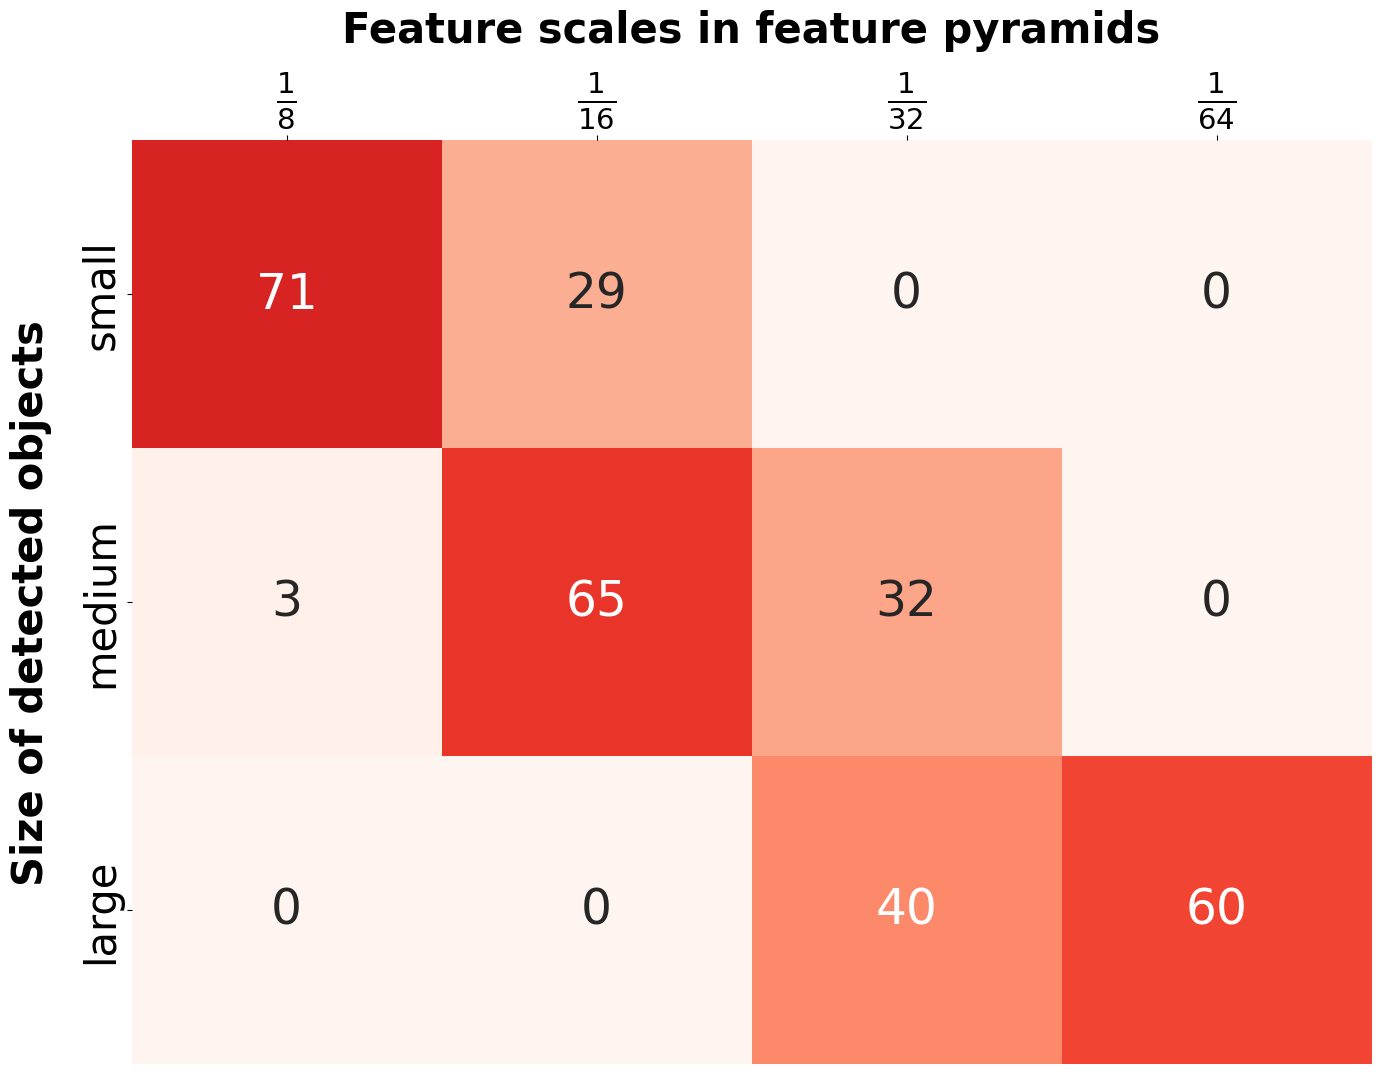
\includegraphics[width=\linewidth]{fig/fpn_vis.png}
%     % }
%     % \subfloat[\label{fig:fpn_comp} \textbf{Feature pyramids are important}, showing a considerable improvement over single-scale input in current detectors.]
%     {
%         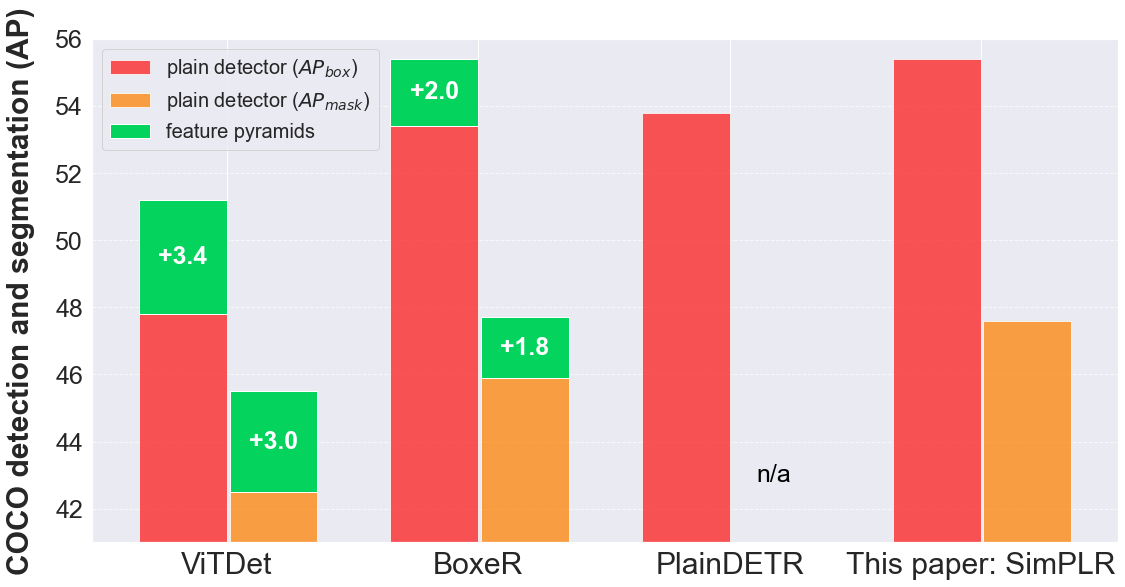
\includegraphics[width=\linewidth]{fig/fpn_comp.png}
%     }
%     \caption{
%     \textbf{A plain detector is non-trivial.} Even with the use of a plain backbone ViT pre-trained using MAE~\cite{he2022mae}, feature pyramids are still important for both convolution-based (ViTDet~\cite{li2022vitdet}) and transformer-based (BoxeR~\cite{nguyen2022boxer}) detectors. While removing multi-scale input from the encoder, PlainDETR~\cite{lin2023plaindetr} still relies on feature pyramids for its box proposal generation and lags behind in performance. In this paper, we demonstrate that the plain detector, \ours, with the proposed scale-aware attention yields competitive performance compared to multi-scale counterparts. %(n/a: PlainDETR is for object detection only).
%     }\label{fig:single_scale}
% \end{figure}

\begin{figure*}[t]
    \centering
    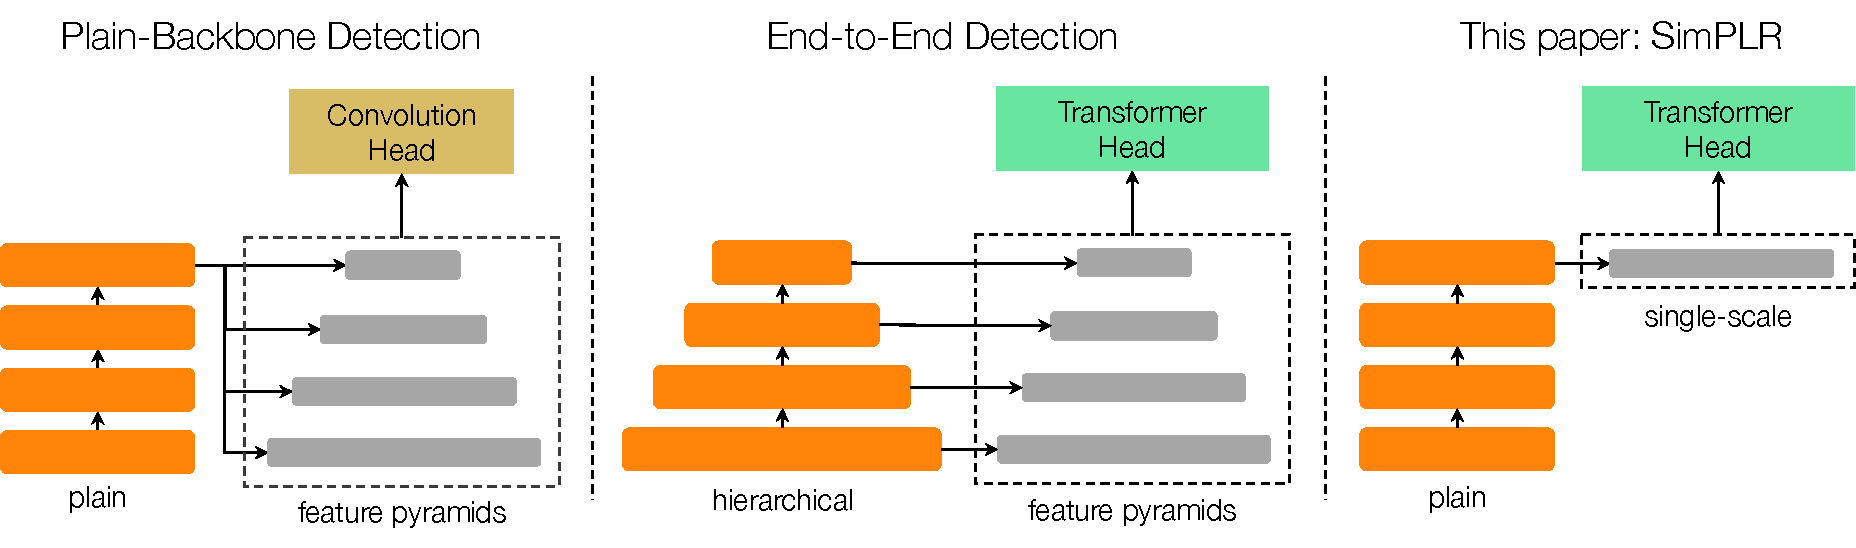
\includegraphics[width=\linewidth]{fig/compare1.pdf}\\
    \caption{
    \textbf{Object detection architectures. Left:} The plain-backbone detector from~\cite{li2022vitdet} whose input (denoted in the dashed region) are multi-scale features. \textbf{Middle:} State-of-the-art end-to-end detectors~\cite{nguyen2022boxer,cheng2022mask2former} utilize a hierarchical backbone (\ie, Swin~\cite{liu2021swintransformer}) to create multi-scale inputs. \textbf{Right:} Our simple single-scale detector following the end-to-end framework. Where existing detectors require feature pyramids to be effective, we propose a plain detector, \ours, whose backbone and detection head are non-hierarchical and operate on a single-scale feature map. The plain detector, \ours, achieves on par or even better performance compared to hierarchical and/or multi-scale counterparts while being more efficient.
    % We show through our experiments that \ours also shows good scaling behaviour and effectively takes advantages from a significant progress of self-supervised learning with ViTs.
    }\label{fig:compare}
\end{figure*}


% \footnotetext{In this paper, ``plain'' refers to the non-hierarchical, single-scale property. The ``plain detector'' is the detector whose backbone and detection head are non-hierarchical and both operate on single-scale features.}

After its astonishing achievements in natural language processing, the transformer \cite{vaswani2017transformer} has quickly become the neural network architecture of choice in computer vision, as evidenced by recent success in image classification \cite{liu2021swintransformer,dosovitskiy2021vit}, object detection \cite{nicolas2020detr,zhu2021deformable,nguyen2022boxer} and segmentation \cite{wang2021maxdeeplab,zhang2021knet,cheng2022mask2former}. Unlike natural language processing, where the same pre-trained network can be deployed for a wide range of downstream tasks with only minor modifications \cite{brown2020gpt3,devlin2019bert}, computer vision tasks such as object detection and segmentation require a different set of domain-specific knowledge to be incorporated into the network. Consequently, it is commonly accepted that a modern object detector contains two main components: a pre-trained backbone as the \emph{general} feature extractor, and a \emph{task-specific} head that conducts detection and segmentation tasks using domain knowledge. For transformer-based vision architectures, the question remains whether to add more inductive biases or to learn them from data.

The spatial nature of image data lies at the core of computer vision. Besides learning long range feature dependencies, the ability of capturing local structure of neighboring pixels is critical for representing and understanding the image content. Building upon the successes of convolutional neural networks, a line of research biases the transformer architecture to be \emph{multi-scale} and \emph{hierarchical} when dealing with the image input, \ie, Swin Transformer \cite{liu2021swintransformer} and others \cite{fan2021mvit,wang2021pvit,heo2021rethinkingvit}.
The hierarchical design makes it easy to create multi-scale features for dense vision tasks and allows pre-trained transformers to be seamlessly integrated into a convolution-based detection head with a feature pyramid network \cite{tsung2017fpn}, yielding impressive results in object detection and segmentation. However, the inductive biases in the architectural design make it benefit less from self-supervised learning and the scaling of model size~\cite{li2022vitdet}.

An alternative direction pursues the idea of a simple transformer with ``less inductive biases'' and emphasizes learning vision-specific knowledge directly from image data. 
Specifically, the Vision Transformer (ViT) \cite{dosovitskiy2021vit} stands out as a \emph{plain} architecture with a constant feature resolution, and acts as the feature extractor in plain-backbone detection. This is motivated by the success of ViTs scaling behaviours in visual recognition \cite{he2022mae,bao2022beit,dehghani2023scalingvit22b}. In addition, the end-to-end detection framework proposed by Carion \etal \cite{nicolas2020detr} with a transformer-based detection head further removes many hand-designed components, like non-maximum suppression or intersection-over-union computation, that encodes the prior knowledge for object detection. 

The plain design of ViTs, however, casts doubts about its ability to capture information of objects across multiple scales. While recent studies \cite{dosovitskiy2021vit,li2022vitdet} suggest that ViTs with global self-attention could potentially learn translation-equivariant and scale-equivariant properties during training, leading object detectors still require multi-scale feature maps and/or an hierarchical backbone. This observation holds true for both convolutional \cite{ren2015faster_rcnn,he2017maskrcnn,li2022vitdet} and transformer-based detectors \cite{zhu2021deformable,nguyen2022boxer,cheng2022mask2former} (see \cref{fig:single_scale}). Unlike hierarchical backbones, the creation of feature pyramids conflicts with the original design philosophy of ViTs. Therefore, our goal is to pursue a plain detector whose backbone \textit{and} detection head are both \textit{single-scale} and \textit{non-hierarchical}. This further simplifies the architecture for detection and segmentation in the pursuit of learning object representations from data.

In this paper, we introduce SimPLR, a plain detector for \textit{both} end-to-end detection and segmentation frameworks~\cite{nicolas2020detr,zhu2021deformable,nguyen2022boxer,cheng2022mask2former}. In particular, our detector extracts the single-scale feature map from a ViT backbone, which is then fed into the transformer encoder-decoder via a simple projection to make the prediction. To deal with objects of various sizes, we propose to incorporate scale information into the attention mechanism, resulting in an \emph{adaptive-scale} attention. The proposed attention mechanism learns to capture adaptive scale distribution from training data. This eliminates the need for multi-scale feature maps from the ViT backbone, yielding a simple and efficient detector.

The proposed detector, \ours, turns out to be an effective solution for the plain detection and segmentation. We find that multi-scale feature maps are not necessary and the scale-aware attention mechanism adequately captures objects at various sizes from output features of a ViT backbone. Despite the plain architecture, our detector (\ours) shows competitive performance compared to the strong hierarchical-backbone or multi-scale detectors (\eg, ViTDet~\cite{li2022vitdet} and Mask2Former~\cite{cheng2022mask2former}), while being consistently faster. Moreover, the effectiveness of our detector is observed not only in object detection but also in instance and panoptic segmentation. Interestingly, the efficient design allows \ours to take advantages of the significant progress in self-supervised learning and scaling with ViTs (\eg, with MAE~\cite{he2022mae} and BEiT~\cite{peng2022beitv2}), indicating plain detectors to be a promising direction for dense prediction tasks.
\section{Related Work}
\label{sec:related_work}

\boldparagraph{Backbones for object detection.} Inspired by R-CNN~\cite{girshick2014rcnn}, modern object detection methods utilize a task-specific head on top of a pre-trained backbone. Initially, object detectors~\cite{simonyan2015vgg,xie2017resnext,kaiming2016resnet,huang2017densenet} were dominated by convolutional neural network (CNN) backbones~\cite{lecun95convolutional} pre-trained on ImageNet~\cite{deng2009imagenet}. With the success of the transformer in learning from large-scale text data~\cite{brown2020gpt3,devlin2019bert}, many studies have explored the transformer for computer vision~\cite{chen2020igpt,dosovitskiy2021vit,liu2021swintransformer}. Most recently, the Vision Transformer (ViT)~\cite{dosovitskiy2021vit} with a simple design demonstrated the capability of learning meaningful representation for visual recognition. By removing the need for labels, methods with self-supervised learning have emerged as an even more powerful solution for pre-training general vision representations~\cite{chen2020simclr,he2022mae}. We show through experiments that \ours can take advantages of the significant progress in representation learning and scaling of ViTs.

% the pre-trained ViT when combined with our proposed encoder-decoder delivers strong performance in detection and segmentation while removing non-trivial adaptations in ViT for feature pyramids.

\boldparagraph{End-to-end detection and segmentation.} The end-to-end framework for object detection proposed in DETR~\cite{nicolas2020detr} aims to remove the need for many hand-crafted modules. This is made possible by adopting Transformer as the detection head to directly give the prediction. Follow-up works~\cite{dong2021solq,wang2021maxdeeplab,nguyen2022boxer} extended the transformer-based head in end-to-end frameworks for instance segmentation, and panoptic segmentation. This inspired MaskFormer~\cite{cheng2021maskformer} and K-Net~\cite{zhang2021knet} to unify segmentation tasks with a class-agnostic mask prediction. Pointing out that MaskFormer and K-Net lag behind specialized architectures, Cheng \etal~~\cite{cheng2022mask2former} introduce Mask2Former, reaching strong performance on segmentation tasks. Yu \etal~\cite{yu2022kmmask} replace self-attention with $k$-means clustering, boosting the effectiveness of the network. Another direction is to improve the object query in the decoder via a denoising process~\cite{zhang2023dino,li2023maskdino}. While simplifying the detection and segmentation framework, these architectures still require an hierarchical backbone along with feature pyramids. The use of feature pyramids increases the sequence length of the input to the transformer-based detection head, making the detector less efficient. In this work, we enable a plain detector by removing hierarchical and multi-scale constraints.

% A universal architecture solves multiple vision tasks without many architectural changes. This is made possible by the introduction of transformers for object detection~\cite{nicolas2020detr}. Follow-up works~\cite{dong2021solq,wang2021maxdeeplab,nguyen2022boxer} extended the end-to-end detection framework to object detection, instance segmentation, and panoptic segmentation. This inspired MaskFormer~\cite{cheng2021maskformer} and K-Net~\cite{zhang2021knet} to unify segmentation tasks with a class-agnostic mask prediction. Pointing out that MaskFormer and K-Net still lag behind specialized architectures,~\cite{cheng2022mask2former} introduce Mask2Former, which outperforms specialized architectures on instance, semantic, and panoptic segmentation. ~\cite{yu2022kmmask} replace self-attention with $k$-means clustering, further boosting the effectiveness of the network. Another direction is to improve the object query in the decoder via a denoising process~\cite{zhang2023dino,li2023maskdino}. Similar to convolution-based detection heads, these approaches utilize multi-scale feature maps from a hierarchical backbone. In this work, we remove the multi-scale feature map constraint and enable \ours on detection and segmentation using a \emph{single-scale} feature map.

\boldparagraph{Plain detectors.} Following the goal of less inductive biases in the architecture, recent studies focus on the non-hierarchical and single-scale detector. Motivated by the success of ViT, a line of research considers plain-backbone detectors that replace the hierarchical backbone with a ViT. Initially, Chen \etal~\cite{chen2022uvit} present UViT as a plain detector that contains a ViT backbone and a single-scale convolutional detection head. Since the backbone architecture is modified \textit{during pre-training} to adopt the progressive window attention, UViT is unable to take the advantages of existing pre-training approaches with ViTs. ViTDet~\cite{li2022vitdet} tackles this problem with simple adaptations of the ViT backbone \textit{during fine-tuning}. These simple modifications allow ViTDet to benefit directly from recent self-supervised learning with ViTs (\ie, MAE~\cite{he2022mae}), resulting in strong results when scaling to larger models. Despite enabling plain-backbone detectors, feature pyramids are still an important factor in ViTDet to detect object at various scales.

Most recently, Lin \etal~\cite{lin2023plaindetr} introduce the transformer-based PlainDETR detector, which also removes the multi-scale input. However, it still relies on multi-scale features to generate the object proposals for its decoder. In the decoder, PlainDETR also uses hybrid matching~\cite{jia2023hybridmatching} to strengthen its prediction, while our decoder preserves a simple design as in~\cite{zhu2021deformable,nguyen2022boxer}. We believe to be the first to remove
the hierarchical and multi-scale constraints which appear in the backbone \textit{and} the input of the transformer encoder for \textit{both} detection and segmentation tasks. Our proposed scale-aware attention can further plug into current end-to-end frameworks without significant architectural changes. %, resulting in a plain detector (\ours).

% Instead, we propose to learn scale information in sparse attention mechanism within our detector (\ours). The scale-aware attention mechanism allows \ours to maintain the single-scale features in both proposal generation and final prediction, yielding a plain detector. We show that \ours demonstrates compelling scaling behavior while being efficient due to the use of sparse attention mechanism.

% Most recently,~\cite{lin2023plaindetr} suggests to remove the use of multi-scale input by designing a transformer-based detection head 

% that a transformer-based detection head with self-attention and box-to-pixel biases gives competitive results on single-scale input from . However, 

% A key challenge in object detection is to detect objects within an image across multiple scales. Early works tackled this problem by applying a CNN detector with a sliding window strategy on an image pyramid~\cite{sermanet2014overfeat} or with generated region proposals~\cite{uijlings2013selective} to extract each scale-normalized region from the input image~\cite{girshick2014rcnn}.
% To reduce computational costs, Faster R-CNN~\cite{ren2015faster_rcnn} generates object proposals on the feature map using a region proposal network. As deeper features of CNNs tends to capture more high-level information at the expense of fine-grained details for small objects, SSD~\cite{wei2016ssd} predicts objects from multiple layers of the feature hierarchy. The Feature Pyramid Network~\cite{tsung2017fpn} further improves the creation of multi-scale feature maps with top-down fusion and lateral connections. With the recent evidence that non-hierarchical transformer architectures (\ie, ViTs) are able to learn convolution-like behaviour through image data (\ie, translation-equivariance), the necessity of multi-scale feature maps becomes questionable. 
% In this study, we demonstrate that a plain ViT backbone along with a single-scale encoder-decoder is able to detect multi-scale objects without the need for feature pyramids.

% \section{Background}
\label{sec:background}
Our goal is to further simplify the detection and segmentation pipeline from~\cite{zhu2021deformable,li2022vitdet,nguyen2022boxer}, and to prove the effectiveness of the plain detector in \textit{both} object detection and segmentation tasks. To do so, we focus on the recent progress in end-to-end detection and segmentation. As a result, we utilize the sparse attention mechanism, Box-Attention in~\cite{nguyen2022boxer}, as strong baselines due to its effectiveness in learning discriminative object representations while being lightweight in computation.

% Given the input feature map from the backbone, the encoder layers with the sparse attention mechanism will output contextual representations. The contextual representations are utilized to predict object proposals and to initialize object queries for the decoder. We denote the input feature map of an encoder layer as $e \in \mathbb{R}^{H_e \times W_e \times d}$ and the query vector $q \in \mathbb{R}^d$, with $H_e, W_e, d$ denoting height, width, and dimension of the input features respectively. 

In box-attention, each query vector $q \in \mathbb{R}^d$ in the input feature map is assigned a reference window $r {=} [x, y, w, h]$, where $x, y$ indicate the query coordinate and $w, h$ are the size of the reference window. The box-attention refines the reference window into a region of interest.
%
% \begin{equation}
%     r' = F_\text{scale}\big(F_\text{translate}(r, q), q\big), 
% \end{equation}
% \begin{equation}
%     F_\text{scale}(r, q) = [x, y, w + \Delta_w, h + \Delta_h], 
% \end{equation}
% \begin{equation}
%     F_\text{translate}(r, q) = [x + \Delta_x, y + \Delta_y, w, h],
% \end{equation}
% %
% where $F_\text{scale}$ and $F_\text{translate}$ are the scaling and translation transformations, $\Delta_x, \Delta_y, \Delta_w$ and $\Delta_h$ are the offsets regarding to the reference window $r$. A linear projection ($\mathbb{R}^d \rightarrow \mathbb{R}^{4}$) is applied on $q$ to predict offset parameters (\ie, $\Delta_x, \Delta_y, \Delta_w$ and $\Delta_h$) \wrt the window size.
%
During the attention head computation, a $2 {\times} 2$ feature grid is sampled from the corresponding region of interest, resulting in a set of value features $v_i \in \mathbb{R}^{2 \times 2 \times d_h}$. The $2 {\times} 2$ attention scores are efficiently generated by computing a dot-product between $q \in \mathbb{R}^d$ and relative position embeddings ($k_i \in \mathbb{R}^{2 \times 2 \times d}$) followed by a $\softmax$ function. The attended feature $\mathrm{head}_i \in \mathbb{R}^{d_h}$ is a weighted sum of $2 {\times} 2$ value features in $v_i$ with the corresponding attention weights:
%
% \begin{equation}
%     \alpha =  \softmax(q^{\top} {k_i}),
% \end{equation}
% \begin{equation}
%     \mathrm{head}_i = \mathop{\mathrm{\boxattnop}}(q, k_i, v_i) = \sum_{j=0}^{2 \times 2} \alpha_j v_{i_j},
% \end{equation}
%
where $q \in \mathbb{R}^d$, $k_i \in \mathbb{R}^{2 \times 2 \times d}$, $v_i \in \mathbb{R}^{2 \times 2 \times d_h}$ are query, key and value vectors of box-attention, $\alpha_j$ is the $j$-th attention weight, and $v_{i_j}$ is the $j$-th feature vector in the feature grid $v_i$. To better capture objects at different scales, the box-attention~\cite{nguyen2022boxer} takes $t$ multi-scale feature maps, $\{e^j\}_{j=1}^t$, as its inputs in order to produce $\mathrm{head}_i$.

% \paragraph{Multi-head Deformable Attention.} In deformable attention, each query vector $q \in \mathbb{R}^d$ is assigned a reference point $p=[x,y]$, where $x,y$ indicate the query coordinate normalized by the image size. The deformable attention attends to points of interest around the query coordinate, $p'$, as:
% %
% \begin{equation}
%     p' = F_\text{deform}(p, q) = [x + \Delta_x, y + \Delta_y],
% \end{equation}
% %
% where $F_\text{deform}$ is the deformable function, $\Delta_x,\Delta_y$ are the offets regarding to the reference point $p$. Similarly, a linear projection ($\mathbb{R}^d \rightarrow \mathbb{R}^2$) is applied on $q$ to predict offset paramters \wrt the reference point.

% During the $i$-th attention head computation, the deformable attention predicts a set of 4 points, resulting in value features $v_i \in \mathbb{R}^{4\times d_h}$. The $4$ attention scores are generated by applying another linear projection, $g_i: \mathbb{R} \rightarrow \mathbb{R}^4$, on $q$ followed by a $\softmax$ function. The attended feature $\mathrm{head}_i \in \mathbb{R}^{d_h}$ is a weighted sum of $4$ value features in $v_i$ with the corresponding attention weights:
% %
% \begin{equation}
%     \alpha =  \softmax\big(g_i(q)\big),
% \end{equation}
% \begin{equation}
%     \mathrm{head}_i = \mathop{\mathrm{\deformattnop}}(q, v_i) = \sum_{j=0}^{4} \alpha_j v_{i_j},
% \end{equation}
% %
% where $q \in \mathbb{R}^d$, $v_i \in \mathbb{R}^{2 \times 2 \times d_h}$ are query, value vectors of deformable attention, $\alpha_j$ is the $j$-th attention weight, and $v_{i_j}$ is the $j$-th feature vector in the value $v_i$. The deformable attention~\cite{zhu2021deformable} also utilizes $t$ multi-scale feature maps, $\{e^j\}_{j=1}^t$, as its inputs in order to produce $\mathrm{head}_i$.


The sparse attention like box-attention and deformable attention lies at the core of recent end-to-end detection and segmentation models due to its ability of capturing object information with lower complexity. The effectiveness and efficiency of these attention mechanisms bring up the question: \textit{Is multi-scale object information learnable within the detector which is non-hierarchical and single-scale?}


\section{\ours: A Simple and Plain Detector}
\label{sec:simplr}

Multi-scale feature maps in a hierarchical backbone can be easily extracted from the pyramid structure~\cite{wei2016ssd,tsung2017fpn,zhu2021deformable}. When moving to a ViT backbone with a constant feature resolution, the creation of multi-scale feature maps requires complex backbone adaptations. Moreover, the benefits of multi-scale features in object detection frameworks using ViTs remain unclear. Recent studies on plain-backbone detection~\cite{li2022vitdet,chen2022uvit} conjecture the high-dimensional ViT with self-attention and positional embeddings~\cite{vaswani2017transformer} is able to preserve important information for localizing objects\footnote{ViT-B and larger ($\text{dim}\ge768$) can maintain information with a patch size of $16{\times}16{\times}3$ in the input image.}. From this conjecture, we hypothesize that a proper design of the transformer-based head will enable a plain detector.

Our proposed detector, \ours, is conceptually simple: a pre-trained ViT backbone to extract plain features from an image, which are then fed into a single-scale encoder-decoder to make the final prediction (See \cref{fig:compare}). Thus, \ours is a natural idea as it eliminates the non-trivial creation of feature pyramids from the ViT backbone. But the single-scale encoder-decoder requires an effective design to deal with objects at different scales. First, we review box-attention in \cite{nguyen2022boxer} as our baseline in end-to-end detection and segmentation using feature pyramids. Then, we introduce the key elements of our plain detector, \ours, including its \emph{scale-aware} attention that is the main factor for learning of adaptive object scales.

\subsection{Background}

Our goal is to further simplify the detection and segmentation pipeline from~\cite{zhu2021deformable,li2022vitdet,nguyen2022boxer}, and to prove the effectiveness of the plain detector in \textit{both} object detection and segmentation tasks. As a result, we utilize the sparse attention mechanism, box-attention in~\cite{nguyen2022boxer}, as strong baselines due to its effectiveness in learning discriminative object representations while being lightweight in computation.

In box-attention, each query vector $q \in \mathbb{R}^d$ in the input feature map is assigned a reference window $r {=} [x, y, w, h]$, where $x, y$ indicate the query coordinate and $w, h$ are the size of the reference window. The box-attention refines the reference window into a region of interest.
During the attention head computation, a $2 {\times} 2$ feature grid is sampled from the corresponding region of interest, resulting in a set of value features $v_i \in \mathbb{R}^{2 \times 2 \times d_h}$. The $2 {\times} 2$ attention scores are efficiently generated by computing a dot-product between $q \in \mathbb{R}^d$ and relative position embeddings ($k_i \in \mathbb{R}^{2 \times 2 \times d}$) followed by a $\softmax$ function. The attended feature $\mathrm{head}_i \in \mathbb{R}^{d_h}$ is a weighted sum of $2 {\times} 2$ value features in $v_i$ with the corresponding attention weights:
%
% \begin{equation}
%     \alpha =  \softmax(q^{\top} {k_i}),
% \end{equation}
% \begin{equation}
%     \mathrm{head}_i = \mathop{\mathrm{\boxattnop}}(q, k_i, v_i) = \sum_{j=0}^{2 \times 2} \alpha_j v_{i_j},
% \end{equation}
%
To capture objects at different scales, the box-attention~\cite{nguyen2022boxer} takes $t$ multi-scale feature maps, $\{e^j\}_{j=1}^t$, as its inputs in order to produce $\mathrm{head}_i$. The multi-scale box-attention shows strong performance in end-to-end object detection and instance segmentation.

The sparse attention like box-attention lies at the core of recent end-to-end detection and segmentation models due to its ability of capturing object information with lower complexity. The effectiveness and efficiency of these attention mechanisms bring up the question: \textit{Is multi-scale object information learnable within the detector which is non-hierarchical and single-scale?}

\subsection{Scale-aware attention}

The output features of the encoder should capture objects at different scales. Therefore, unlike the feature pyramids where each set of features encode a specific scale, predicting objects from a plain feature map requires its feature vectors to reason about dynamic scale information based on the image content. This can be addressed effectively by a multi-head attention mechanism that capture different scale information in each of its attention heads. 
In that case, global self-attention is a potential candidate because of its large receptive field and powerful representation. However, its computational complexity is quadratic \wrt the sequence length of the input, making the operation computationally expensive when dealing with high-resolution images. The self-attention also leads to worse performance and slow convergence in end-to-end detection~\cite{zhu2021deformable}. This motivated us to develop a multi-head \emph{scale-aware} attention mechanism for single-scale input.

\boldparagraph{Scale-aware attention.} In the sparse attention mechanism such as deformable attention~\cite{zhu2021deformable} or box-attention~\cite{nguyen2022boxer}, each feature vector is assigned to a single scale in feature pyramids. As a result, feature vectors learn to adapt to that specific scale assigned to them. While this behaviour may not impact the multi-scale deformable attention or box-attention -- which utilizes feature pyramids for detecting objects -- it poses a big challenge in learning scale-equivariant features on a single-scale input.

To address this limitation, we propose two variants of multi-head \emph{scale-aware} attention (\ie, \emph{fixed-scale} and \emph{adaptive-scale}) that integrate different scales into each attention head, allowing query vectors to choose the suitable scale information during training. Our proposed attention mechanism is simple: we assign reference windows of $m$ different scales to attention heads of each query. We use $m$ reference windows with size $w {=} h \in \{s \cdot 2^j\}_{j=0}^{m-1}$, where $s$ is the size of the smallest window, and $m$ is the number of scales. Surprisingly, our experiments show that the results are \emph{not} sensitive to the size of the window, as long as \emph{enough number of scales} are used.
%
\begin{enumerate}[leftmargin=*,itemsep=0pt,topsep=0pt]
    \item[i)] \emph{Fixed-Scale Attention.} Given reference windows of $m$ scales, we distribute them to $n$ attention heads in a round-robin manner. Thus, in multi-head fixed-scale attention, $\frac{n}{m}$ attention heads are allocated for each of the window scales. This uniform distribution of different scales enables fixed-scale attention to learn diverse information from local to more global context. The aggregation of $n$ heads results in scale-aware features, that is suitable for predicting objects of different sizes.
    \item[ii)] \emph{Adaptive-Scale Attention.} Instead of uniformly assigning $m$ scales to $n$ attention heads, the adaptive-scale attention learns to allocate a scale distribution based on the context of the query vector. This comes from the motivation that the query vector belonging to a small object should use more attention heads for capturing fine-grained details rather than global context, and vice versa. 
    
    % More specifically, in each attention head, the adaptive-scale attention predicts offsets for all reference windows of $m$ scales and samples feature grids from $m$ regions-of-interest. 
    % Given the query vector $q \in \mathbb{R}^d$, it then applies a learnable projection on $q$ followed by $\softmax$ normalization to generate attention scores which allow it to focus on the feature grid of suitable scale. The adaptive-scale attention provides efficiency due to sparse sampling and strong flexibility to control scale distribution via its attention computation.
    Given the query vector $q \in \mathbb{R}^d$ in the input feature map and $m$ reference windows of different scales, $\{r^j\}_{j=0}^{m-1}$, the adaptive-scale attention predicts offsets of all reference windows, $\{\Delta_{x_j},\Delta_{y_j},\Delta_{w_j},\Delta_{h_j}\}_{j=0}^{m-1}$, in each attention head. Besides, we apply a scale temperature to each set of offsets before the transformations:
    \begin{equation}
        F_\text{scale}(r_j, q) = [x, y, w + \Delta_w\cdot\frac{2^j}{\lambda}, h + \Delta_h\cdot\frac{2^j}{\lambda}], 
    \end{equation}
    \begin{equation}
        F_\text{translate}(r_j, q) = [x + \Delta_x\cdot\frac{2^j}{\lambda}, y + \Delta_y\cdot\frac{2^j}{\lambda}, w, h],
    \end{equation}
    where $\frac{2^j}{\lambda}$ is the scale temperature corresponding to $r_j$. The scale temperature allows the transformation functions to capture regions of interest corresponding to the scale of reference windows. It then samples feature grids from $m$ regions of interest and generates attention scores for these feature grids followed by $\softmax$ normalization. This makes our attention mechanism to focus on feature grids of suitable scale. The adaptive-scale attention provides efficiency due to sparse sampling and strong flexibility to control scale distribution via its attention computation.
\end{enumerate}

\subsection{Object Representation for Panoptic Segmentation} 

Panoptic segmentation proposed by~\cite{kirillov2019panoptic} requires the network to segment both ``thing'' and ``stuff''. To enable the plain detector on panoptic segmentation, we make an adaptation in the mask prediction of \ours. Following~\cite{cheng2022mask2former}, we predict segmentation masks of both types by computing the dot-product between object queries and a high-resolution feature map (\ie, $\frac{1}{4}$ feature scale).

As the ViT and SimPLR encoder features are of lower resolution, we simply interpolate the last encoder layer to $\frac{1}{4}$ scale and add a single scale-aware attention layer on top. This simple modification produces a high resolution feature map that is beneficial for learning fine-grained details.

\begin{figure}[t]
\floatbox[{\capbeside\thisfloatsetup{capbesideposition={right,top},capbesidewidth=4cm}}]{figure}[\FBwidth]
{\caption{
    \textbf{Masked Instance-Attention. Left:} The box-attention~\cite{nguyen2022boxer} which samples $2\times2$ grid features in the region of interest. \textbf{Right:} Our masked instance-attention for dense grid sampling. The $2\times2$ attention scores are denoted in four colours and the masked attention scores are in white.}
    \label{fig:masked_instance_attn}}%
{
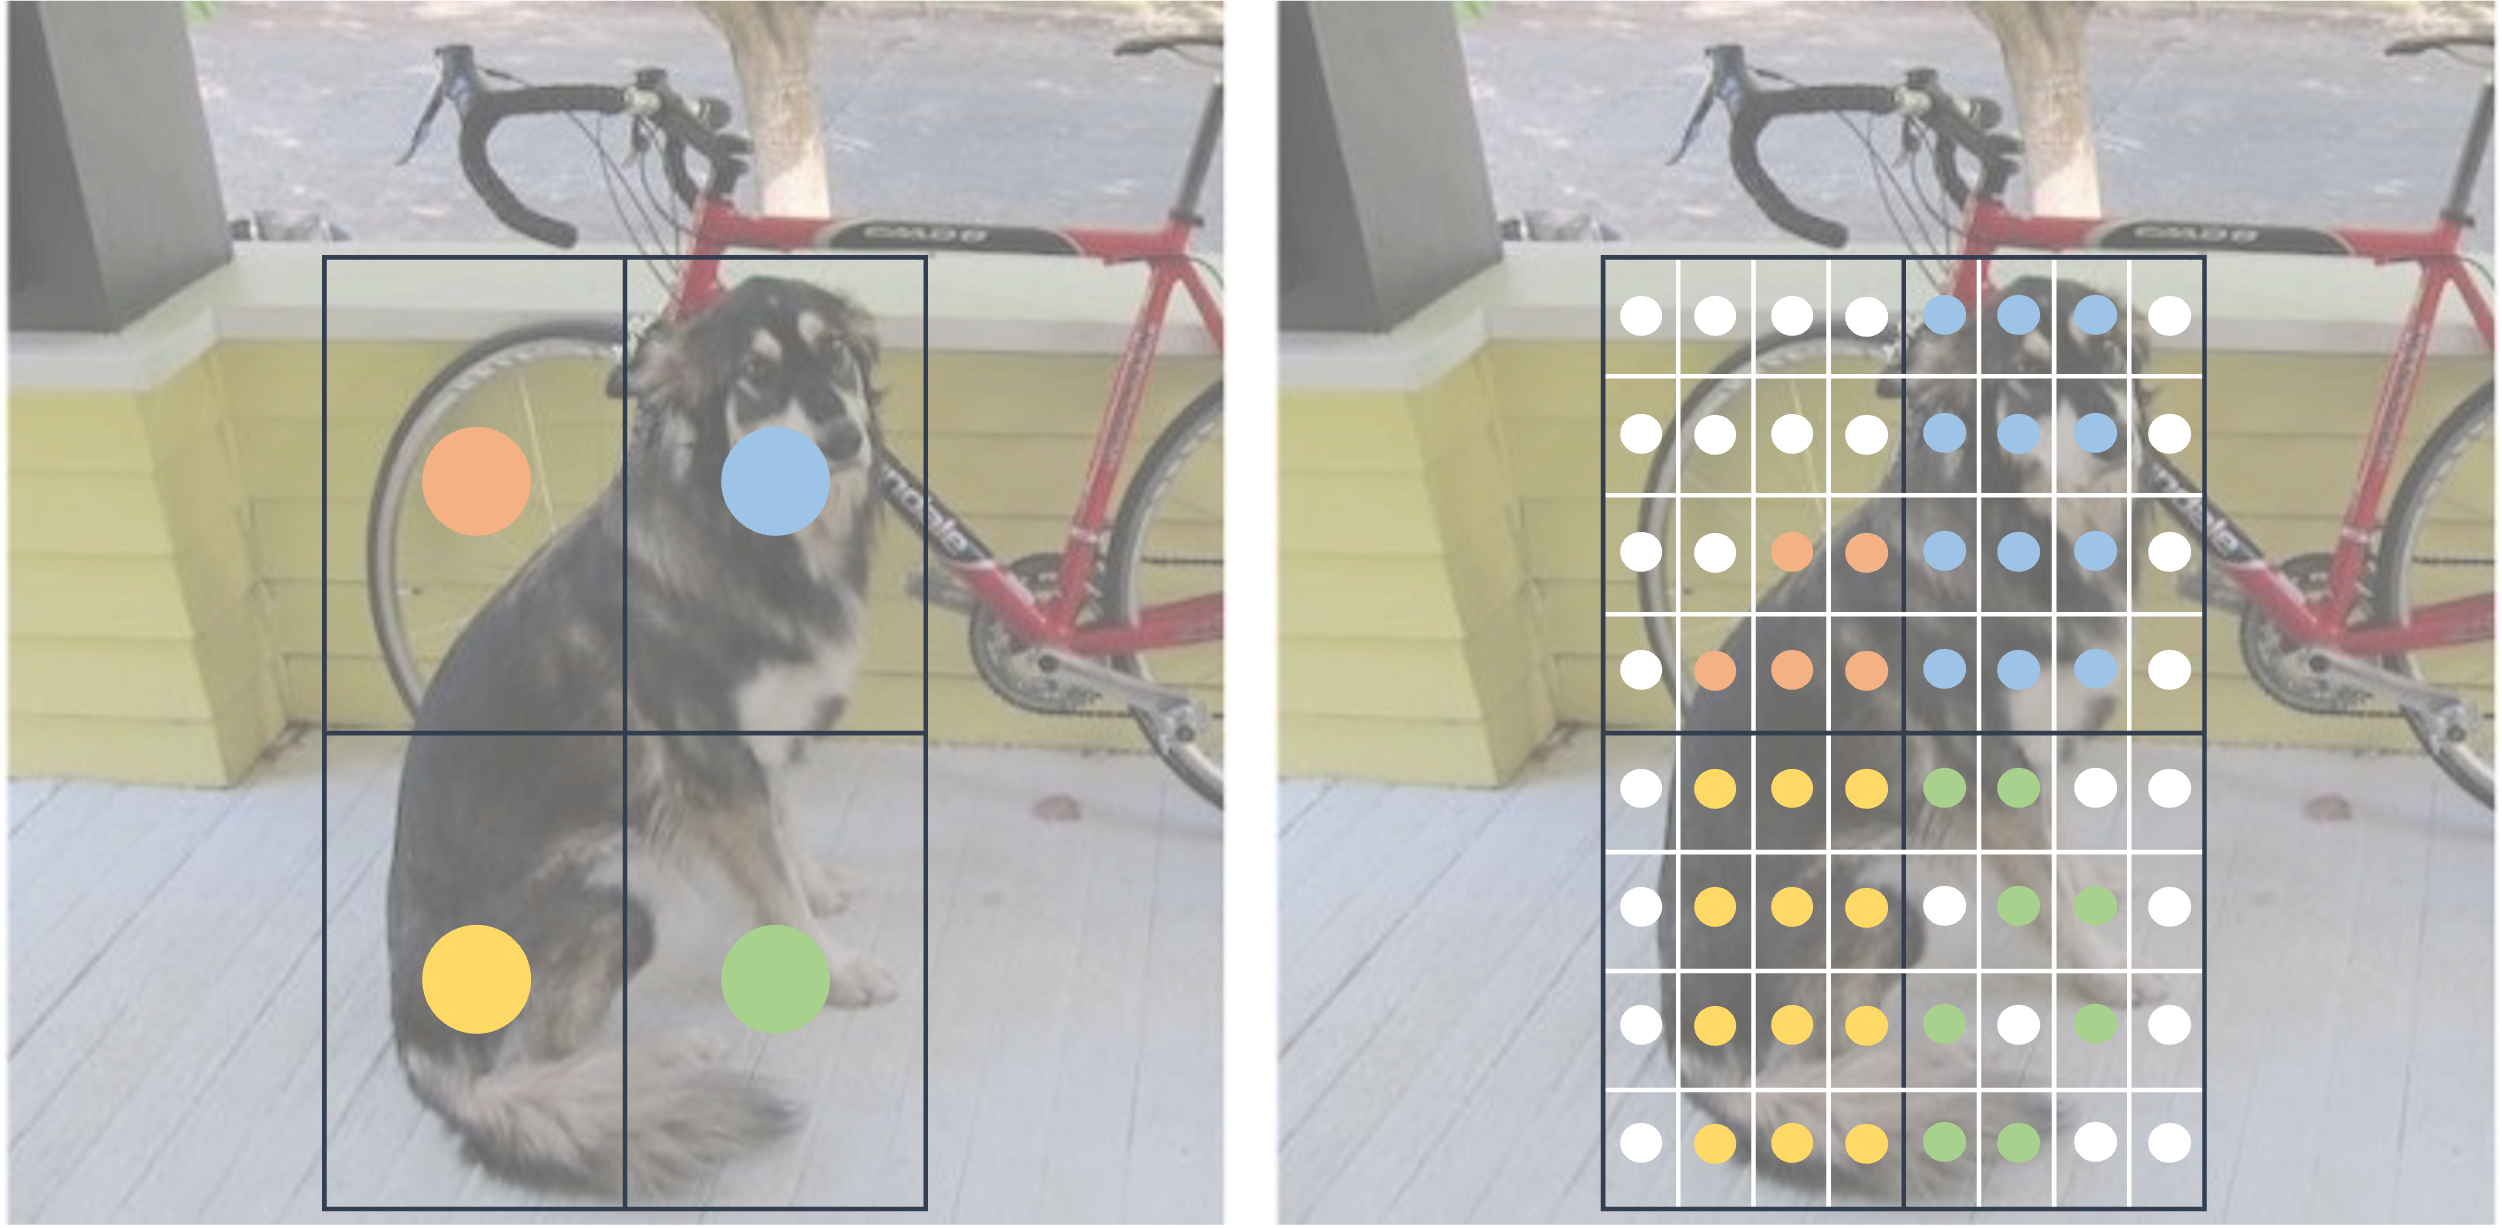
\includegraphics[width=7.5cm]{fig/attn_comp.png}
}
\end{figure}

\boldparagraph{Masked instance-attention.} In order to learn better object representation in the decoder, we propose masked instance-attention that is also a sparse attention mechanism for efficiency. The masked instance-attention follows the grid sampling strategy of the box-attention in~\cite{nguyen2022boxer}, but improves the attention computation to better capture objects of
different shapes.

To be specific, the region of interest $r'_i$ is divided into 4 bins of $2 \times 2$ grid, each of which contains a $\frac{m}{2} \times \frac{m}{2}$ grid features sampled using bilinear interpolation. Instead of assigning an attention weight to each feature vector, a linear projection ($\mathbb{R}^d \rightarrow \mathbb{R}^{2 \times 2}$) is adopted to generate the $2 \times 2$ attention scores for 4 bins. The $\frac{m}{2} \times \frac{m}{2}$ feature vectors within the same bin share the same attention weight. Inspired by \cite{cheng2022mask2former}, we utilize the mask prediction of the previous decoder layer as the attention mask to guide the attention scores to better capture the boundary of objects (see \cref{fig:masked_instance_attn}).
\begin{equation}
    \mathrm{head}_i = \sum_{k=0}^{2 \times 2} \sum_{j=0}^{\frac{m}{2} \times \frac{m}{2}} \frac{\alpha_k}{\frac{m}{2} \cdot \frac{m}{2}} \, v_{i_{k,j}},
\end{equation}
where $a_k$ is the attention weight corresponding to $k$-th bin, $v_{i_{k,j}}$ is the $j$-th feature vector inside $k$-th bin.

\subsection{Network Architecture}

\ours follows the end-to-end detection and segmentation framework in~\cite{nguyen2022boxer} with the two-stage design. Specifically, we use a plain ViT as the backbone with $14\times14$ windowed attention and four equally-distributed global attention blocks as in~\cite{li2022vitdet}. In the detection head, the \ours encoder receives input features via a projection of the last feature map from the ViT backbone. The object proposals are then generated using single-scale features from the encoder and top-scored features are initialized as object queries for the \ours decoder to predict bounding boxes and masks. 

Formally, we apply a projection $f$ to the last feature map of the pre-trained ViT backbone, resulting in the input feature map $e \in \mathbb{R}^{H_e \times W_e \times d}$ where $H_e, W_e$ are the size of the feature map, and $d$ is the hidden dimension of the detection head. In \ours, the projection $f$ is simply a single convolution projection, that provides us a great flexibility to control the resolution and dimension of the input features $e$ to the encoder. The projection allows \ours to decouple the feature scale and dimension between its backbone and detection head to further improve the efficiency. This practice is different from the creation of SimpleFPN in~\cite{li2022vitdet} where a different stack of multiple convolution layers is used for each feature scale (more details shown in Fig. A in the supplementary material). We show by experiments that this formulation is key for plain detection and segmentation while keeping our network efficient.

\boldparagraph{Plain backbone.} \ours deploys ViT as its plain backbone for feature extraction. We show that \ours can take advantages of recent progress in self-supervised learning with ViTs. To be specific, \ours generalizes to ViT backbones initialized by MAE~\cite{he2022mae} and BEiTv2~\cite{peng2022beitv2}. The efficient design of \ours allows us to effectively scale to larger ViT backbones which recently show to be even more powerful in learning representations~\cite{he2022mae,zhai2022scalingvit,dehghani2023scalingvit22b}. We provide more details in the supplementary material.


\section{Experiments}
\label{sec:experiments}

\boldparagraph{Experimental setup.} In this study, we evaluate our method on COCO~\cite{lin2014mscoco}, a commonly used dataset for object detection, instance segmentation, and panoptic segmentation tasks. By default, we use plain features with adaptive-scale attention as described in \cref{sec:simplr} due to its strong performance and ability to perform both detection and segmentation; and initialize the ViT backbone from MAE~\cite{he2022mae} pre-trained on ImageNet-1K without any labels. In both fixed-scale and adaptive-scale attention, we set the number of scale $m=4$ and the window size $s=32$. Unless specified, the hyper-parameters are the same as in \cite{nguyen2022boxer}.

For all experiments, our optimizer is AdamW~\cite{loshchilov2019adamw} with a learning rate of 0.0001. The learning rate is linearly warmed up for the first 250 iterations and decayed at 0.9 and 0.95 fractions of the total number of training steps by a factor 10. ViT-B~\cite{dosovitskiy2021vit} is set as the backbone. The input image size is $1024\times1024$ with large-scale jitter \cite{shiasi2021lsjitter} between a scale range of $[0.1, 2.0]$. We employ query denoising~\cite{zhang2023dino} when compared with other methods. Due to the limit of our computational resources, we report the ablation study using the standard $5\times$ schedule setting with a batch size of 16 as in \cite{nguyen2022boxer}. In the main experiments, we use the finetuning recipe from \cite{li2022vitdet}.

% \boldparagraph{A single-scale detector is non-trivial.} We first study the effect of the scaling transformation in box-attention on feature pyramids as it could possibly generate regions-of-interest at different scales. More specifically, we compare the area between generated regions and the initial reference window of query vectors corresponding to object proposals in the last encoder layer. Surprisingly, the change of area after scaling has a mean of 31\% and standard deviation 33\% \wrt the original area of the reference window (\eg, for a reference window of $32\times32$ pixels to capture regions of different scales, such as $64\times64$ or $16\times16$ pixels, the change of the area should be more than 75\%). This suggests that the scaling function in box-attention prefers to capture regions of different aspect ratios rather than multi-scale information. 

% It can be seen in \cref{fig:single_scale} that deploying feature pyramids brings a large improvement to different types of detectors (\ie, $\sim$2 AP points for BoxeR and $\sim$3 AP points for ViTDet). This observation is consistent to the observation in DeformableDETR \cite{zhu2021deformable} where the improvement of $\sim$2 AP points comes from feature pyramids. While removing multi-scale input to the detection head, the PlainDETR~\cite{lin2023plaindetr} still depends on features pyramids to generate object proposals, their performance drops by $\sim$1 AP when using single-scale features for proposal generation.

\begin{table}[t]
    {
    \centering
    \footnotesize
    {
    \tablestyle{6pt}{1.2}
    \begin{tabular}{lccc}
    \multicolumn{1}{l|}{} & \multicolumn{1}{c|}{\multirow{2}{*}{FPS}} & \multicolumn{1}{c}{\multirow{2}{*}{AP$^\text{b}$}} & \multicolumn{1}{c}{\multirow{2}{*}{$\text{AP}^\text{m}$}} \\
    \multicolumn{1}{l|}{} &  \multicolumn{1}{c|}{} &  \multicolumn{1}{c}{} &  \\
    \shline
    \rowcolor{orange!50} \textbf{Feature pyramids} &  &  & \\
    \multicolumn{1}{l|}{DETR reported in~\cite{lin2023plaindetr}} & \multicolumn{1}{c|}{-} & 46.5 & n/a \\
    \multicolumn{1}{l|}{DeformableDETR reported in~\cite{lin2023plaindetr}} & \multicolumn{1}{c|}{12} & 52.1 & n/a \\
    \multicolumn{1}{l|}{DeformableDETR (our impl.)} & \multicolumn{1}{c|}{12} & 54.6 & n/a \\
    \multicolumn{1}{l|}{BoxeR~\cite{nguyen2022boxer}} &  \multicolumn{1}{c|}{12} & 55.4 & 47.7 \\
    \multicolumn{1}{l|}{ViTDet w/ Cascade head~\cite{li2022vitdet}} & \multicolumn{1}{c|}{11} & 54.0 & 46.7 \\
    \hline
    \rowcolor{orange!50} \textbf{Plain detector} &  &  & \\
    \multicolumn{1}{l|}{PlainDETR$^\dag$~\cite{lin2023plaindetr}} & \multicolumn{1}{c|}{12} & 53.8 & n/a \\
    \multicolumn{1}{l|}{{\ours}} & \multicolumn{1}{c|}{\bf 17} & {\bf 55.7} & {\bf 47.9}  \\
    \end{tabular}
    }
    \begin{tablenotes}
    \centering
    \item[] $\dag$: Multi-scale features are used to generate object proposals.
    \end{tablenotes}
    % \vspace{1em}
    {\caption{\textbf{\ours is an effective plain detector.} All methods use ViT-B as backbone. Methods that take feature pyramids as input employ SimpleFPN with ViT from \cite{li2022vitdet}. Our plain detector, \ours, shows competitive performance compared to multi-scale alternatives, while being faster during inference.}\label{tab:compare}}%
    }
\end{table}

\begin{table}[t]
    \begin{minipage}{\linewidth}
        \centering
        \footnotesize
        \subfloat[\label{tab:strat} \textbf{Scale-aware attention.}]
        {
        \tablestyle{5pt}{1.2}
        \begin{tabular}{l|cc}
        attention & AP$^\text{b}$ & $\text{AP}^\text{m}$ \\
        \shline
        base & 53.6 & 46.1 \\
        \hline
        i) fixed-scale & 55.0 & 47.2 \\
        \rowcolor{orange!25} ii) adaptive-scale & 55.4 & 47.6 \\
        & & \\
        \end{tabular}
        }
        \hspace{2mm}
        \subfloat[\label{tab:window_size} \textbf{Window size.}]
        {
        \tablestyle{5pt}{1.2}
        \begin{tabular}{l|cc}
        $s$ & AP$^\text{b}$ & $\text{AP}^\text{m}$ \\
        \shline
        base & 53.6 & 46.1 \\
        \hline
        16 & 55.1 & 47.4 \\
        \rowcolor{orange!25} 32 & 55.4 & 47.6 \\
        64 & 55.1 & 47.4 \\
        \end{tabular}
        }
        \hspace{2mm}
        \subfloat[\label{tab:num_scale} \textbf{Number of window scales}.]
        {
        \tablestyle{9pt}{1.2}
        \begin{tabular}{l|cc}
        $n$ & AP$^\text{b}$ & $\text{AP}^\text{m}$ \\
        \shline
        base & 53.6 & 46.1 \\
        \hline
        2 & 54.6 & 47.0 \\
        \rowcolor{orange!25} 4 & 55.4 & 47.6 \\
        6 & 55.2 & 47.6 \\
        \end{tabular}
        }

        \subfloat[\label{tab:feat_scale} \textbf{Scales of input features.}]
        {
        \tablestyle{6.5pt}{1.2}
        \begin{tabular}{l|cc}
        scale & AP$^\text{b}$ & $\text{AP}^\text{m}$ \\
        \shline
        base & 53.6 & 46.1 \\
        \hline
        1/4 & 55.4 & 47.7 \\
        \rowcolor{orange!25} 1/8 & 55.4 & 47.6 \\
        1/16 & 54.3 & 46.7 \\
        \end{tabular}
        }
        \hspace{5mm}
        \subfloat[\label{fig:attn_vis} Visualization of scale distribution learnt in \textbf{multi-head adaptive-scale attention} of object proposals. Objects are classified into \emph{small}, \emph{medium}, and \emph{large} based on their area.]
        {
        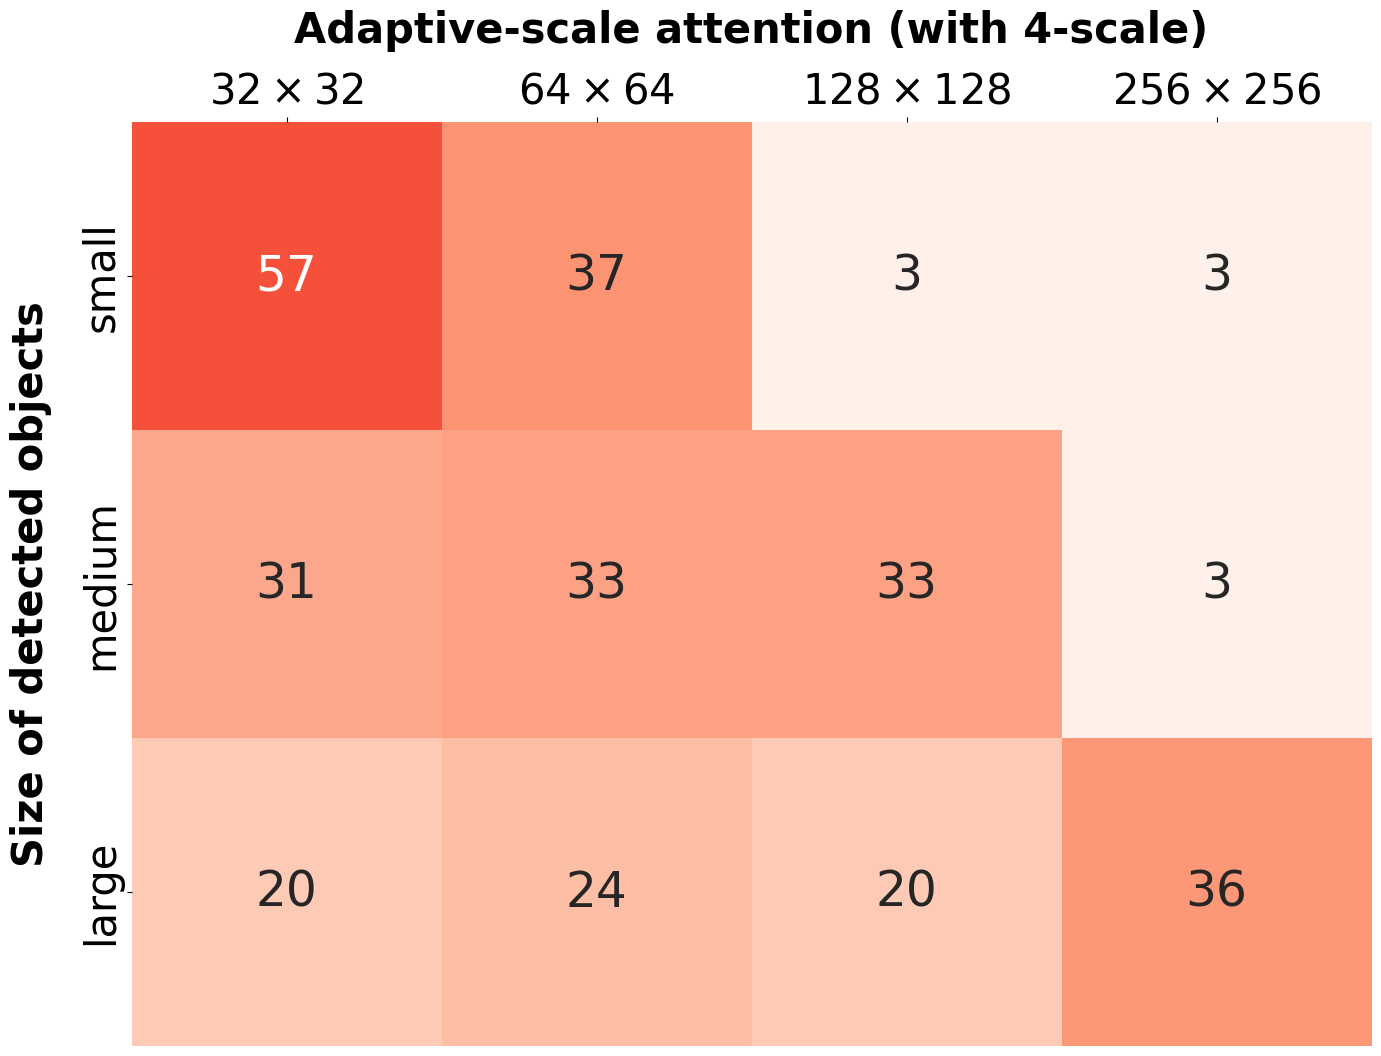
\includegraphics[width=0.46\textwidth]{fig/adaptive_scale.png}
        }
    \end{minipage}
    % \setcounter{table}{2}
    % \setcounter{subtable}{4}
    % \begin{minipage}{0.4\linewidth}
    %     \centering
    %     % \vspace*{1mm}
    %     \subfloat[\label{fig:attn_vis} Visualization of scale distribution learnt in \textbf{multi-head adaptive-scale attention} of object proposals. Objects are classified into \emph{small}, \emph{medium}, and \emph{large} based on their area.]
    %     {
    %     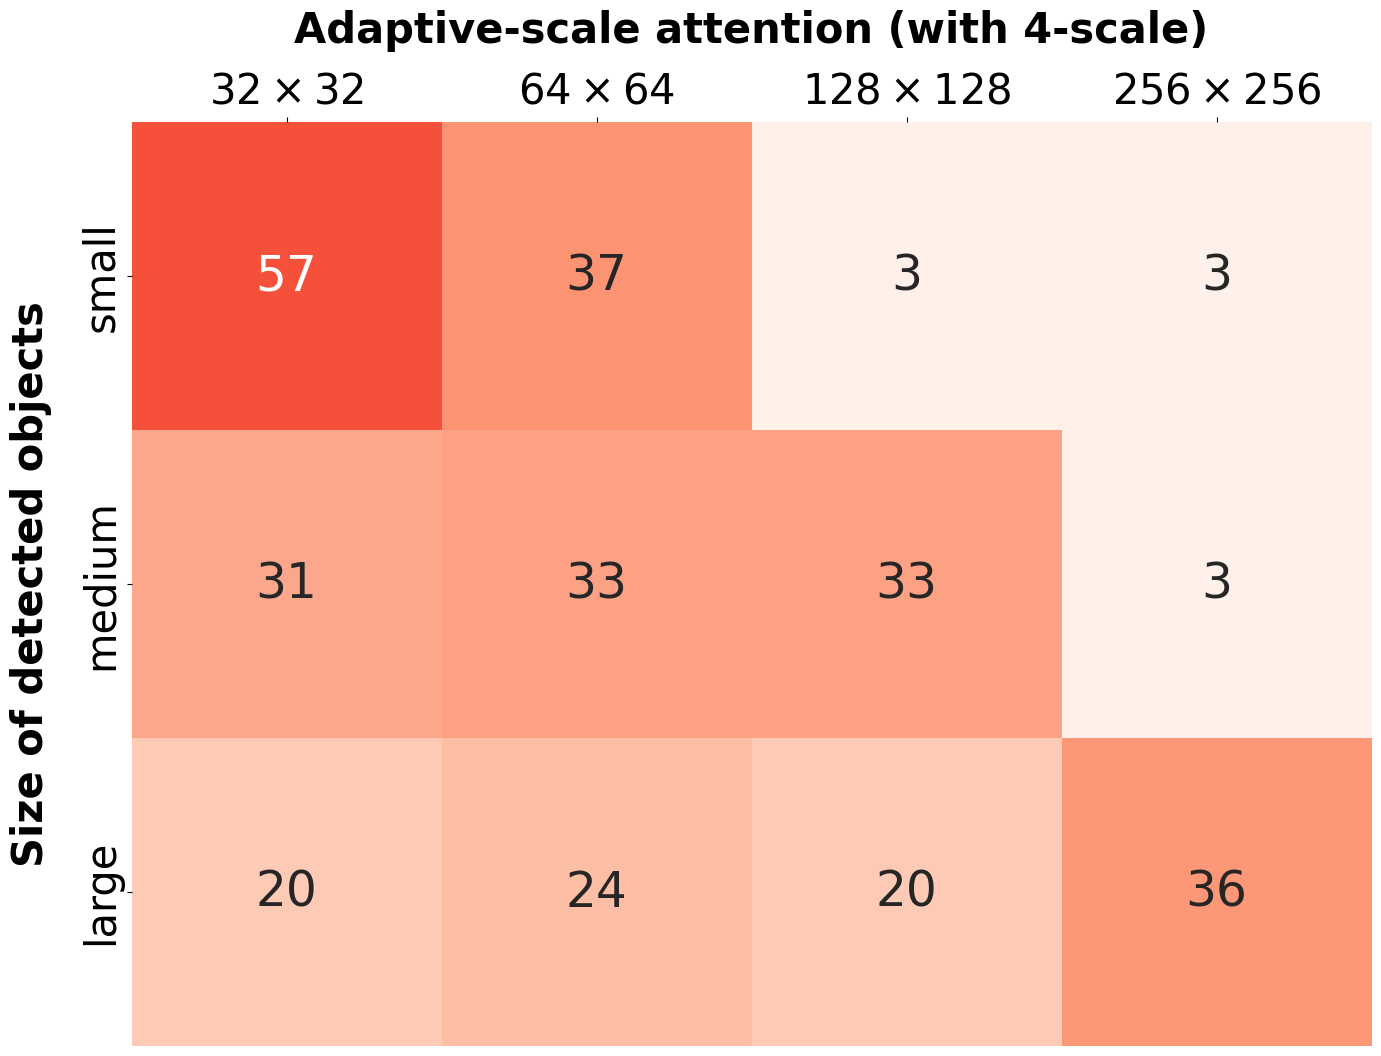
\includegraphics[width=\textwidth]{fig/adaptive_scale.png}
    %     }
    % \end{minipage}
    % \setcounter{table}{2}
    \caption{\label{tab:det_ablation} \textbf{Ablation of scale-aware attention} in \ours using a plain ViT backbone on COCO~\val. \textbf{Table (a-d):} Compared to the na\"ive baseline, which employs BoxeR and box-attention \cite{nguyen2022boxer} with \textit{single-scale} features, our plain detector, \ours, with scale-aware attention improves the performance consistently for all settings, default setting highlighted. 
    \textbf{Figure e:} our adaptive-scale attention captures different scale distribution in its attention heads based on the context of query vectors. Specifically, queries of \emph{small} objects tends to focus on reference windows of small scales (\ie, mainly \(32\times32\)), while query vectors of \emph{medium} and \emph{large} objects distribute more attention computation into larger reference windows. All experiments are with $5\times$ schedule.}
\end{table}

\boldparagraph{\ours is an effective single-scale detector.} In \cref{tab:compare}, we show the comparison between \ours and recent object detectors using the plain backbone ViT. We also implement a strong baseline of DeformableDETR~\cite{zhu2021deformable} with SimpleFPN under our end-to-end framework for better comparison. The plain detector, \ours, with both scale-aware box-attention (SAB) and scale-aware deformable attention (SAD) removes the need for multi-scale adaptation of the ViT.

While \ours with scale-aware deformable attention lags behind its multi-scale counterpart from our implementation, we observe a much smaller gap compared to standard deformable attention on single-scale input (\eg, 0.3 \vs 2 AP point). When equipped with scale-aware box-attention, \ours reaches similar performance as BoxeR and outperforms other multi-scale detectors in both detection and segmentation. In addition, the plain detector is more efficient than multi-scale counterparts. When moving to larger models with higher dimension, we find that multi-scale detectors like BoxeR require significant memory optimization and becomes challenging for our computational resources. We also compare with PlainDETR~\cite{lin2023plaindetr} which is a recent plain detection method. As discussed in \cref{sec:related_work}, PlainDETR and our work approach the plain detector in different ways. PlainDETR aims at designing a strong decoder that compensates for single-scale input, while our goal is to learn scale equivariant features in backbone and encoder. Despite the different approaches, both PlainDETR and our work indicate that plain detection holds a great potential.

% \cref{tab:compare} indicates that \ours with single-scale input outperforms ViTDet and reaches competitive performance compared to BoxeR. This is different from recent object detectors with transformers \cite{zhu2021deformable,cheng2022mask2former} in which multi-scale feature maps are needed to achieve strong performance for both object detection and segmentation.
% In contrast, our experiment demonstrates that single-scale features are sufficient and the proposed design of \ours allows features to learn suitable scale information for detecting objects of various scales. We find that the significance of multi-scale feature maps diminishes when the encoder is equipped with a powerful attention mechanism.


% %%%%%%%%%%%%%%%%%%%%%%%%%%%%%%%%%%%%%%%%%%%%%%%%%%%%%%%%%%%%%%%%%%%%
% \begin{figure}[b]
% \centering

% \begin{minipage}{1\linewidth}
% \centering

% \begin{minipage}[b]{.49\linewidth}
% 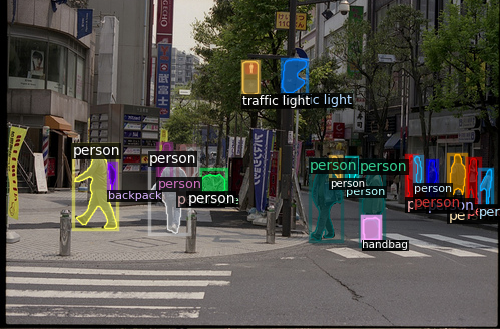
\includegraphics[width=\linewidth]{vis/success/val_848_det.png}
% \end{minipage}
% \begin{minipage}[b]{.49\linewidth}
% 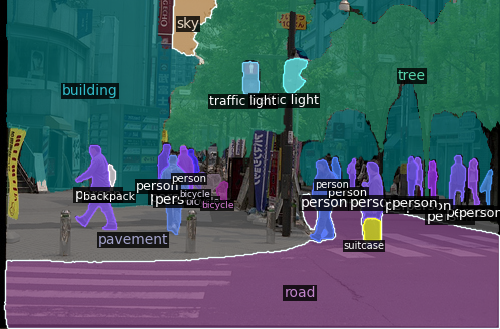
\includegraphics[width=\linewidth]{vis/success/val_848_pan.png}
% \end{minipage}

% \end{minipage}

% \caption{\textbf{Qualitative results} for object detection, segmentation and panoptic segmentation on COCO \val as generated by \ours with ViT-B backbone. \ours can detect and segment objects in crowded scenes.}
% \label{fig:vis}
% % \vspace{-0.2in}
% \end{figure}
% %%%%%%%%%%%%%%%%%%%%%%%%%%%%%%%%%%%%%%%%%%%%%%%%%%%%%%%%%%%%%%%%%%%%

\boldparagraph{Ablation of scale-aware attention.} Here, our baseline is the standard box-attention from \cite{nguyen2022boxer} with single-scale feature input directly taken from the last feature of the ViT backbone (denoted as ``base''). 

From \cref{tab:strat}, we first conclude that \emph{both} scale-aware attention strategies are substantially better than the na\"ive baseline, increasing AP by up to 1.8 points. We note that while fixed-scale attention distributes 25\% of its attention heads into each of the window scales, adaptive-scale attention decides the scale distribution based on the query content. By choosing feature grids from different window scales adaptively, the adaptive-scale attention is able to learn a suitable scale distribution through training data, yielding better performance compared to fixed-scale attention. This is also verified in Fig.~\ref{fig:attn_vis} where queries corresponding to \emph{small} objects tend to pick reference windows of small sizes for its attention heads. Interestingly, queries corresponding to \emph{medium} and \emph{large} objects pick not only reference windows of their sizes, but also ones of smaller sizes. One of reasons may come from the fact that performing instance segmentation of larger objects still requires the network to faithfully preserve the per-pixel spatial details.

In \cref{tab:window_size}, we compare the performance of \ours across several sizes ($s$) of the reference window. They all improve over the baseline, while the choice of a specific base size makes only marginal differences. Our ablation reveals that the number of scales rather than the window size plays an important role to make our network more \emph{scale-aware}. Indeed, in \cref{tab:num_scale}, the use of 4 or more window scales shows improvement up to 0.8 AP over 2 window scales; and clearly outperforms the na\"ive baseline. Last, we show in \cref{tab:feat_scale} that the \emph{decouple} between feature scale and dimension of the ViT backbone and the detection head features helps to boost the performance of our plain detector by $\sim$1 AP point, while keeping its efficiency (\ie, both in terms of FLOPs and FPS). This practice makes scaling of \ours to larger ViT backbones more practical.

\boldparagraph{Ablation on more pre-training data and strategies.} \cref{tab:pretrain} compares the ViT backbone when pre-trained using different strategies with different sizes of pre-training data. \ours with the ViT backbone benefits from better pre-training methods even with supervised approaches. Among supervised pre-training methods, DEiTv3~\cite{touvron2022deit3} shows better results than DEiT~\cite{touvron2021deit}, and the pre-training on more data (\ie, ImageNet-21K) further improves the performance of DEiTv3.
  
However, self-supervised methods like MAE~\cite{he2022mae} provides strong pre-trained backbones when only pre-trained on ImageNet-1K. The best performance is reported with self-supervised method, BEiTv2~\cite{peng2022beitv2} with more pre-training data of ImageNet-21K. This further confirms that our plain detector, \ours, enjoys the significant progress of self-supervised learning and scaling ViTs with data. A similar observation is also pointed out in ViTDet~\cite{li2022vitdet} where the plain ViT backbone initialized with MAE shows better improvement over hierarchical backbones.

%%%%%%%%%%%%%%%%%%%%%%%%%%%%%%%%%%%%%%%%%%%%%%%%%%%%%%%%%%%%%%%%%%%
\begin{table}[t]
    \centering
    \footnotesize
    {
    \tablestyle{7pt}{1.2}
    \begin{tabular}{l|cccc|cccc}
    \multirow{2}{*}{pre-train} & \multicolumn{4}{c|}{Object Detection} & \multicolumn{4}{c}{Instance Segmentation} \\
    & AP$^\text{b}$ & AP$^\text{b}_\text{S}$ & AP$^\text{b}_\text{M}$ & AP$^\text{b}_\text{L}$ & $\text{AP}^\text{m}$ & $\text{AP}^\text{m}_\text{S}$ & $\text{AP}^\text{m}_\text{M}$ & $\text{AP}^\text{m}_\text{L}$ \\
    % \hshline
    % (dynamic)  & \cmark & \xmark & \cmark & \xmark & \cmark & \xmark & \cmark \\
    \shline
    IN-1K, DEiT & 53.6 & 33.7 & 58.1 & 71.5 & 46.1 & 24.5 & 50.4 & 67.2 \\
    IN-1K, DEiTv3 & 54.0 & 34.3 & 58.8 & 70.5 & 46.4 & 24.8 & 51.1 & 66.7 \\
    IN-21K, DEiTv3 & 54.8 & 35.4 & 59.0 & {\bf 72.4} & 47.1 & 25.8 & 51.2 & 68.5 \\
    \hline
    IN-1K, MAE & 55.4 & 36.1 & 59.1 & 70.9 & 47.6 & {\bf 26.8} & 51.4 & 67.1 \\
    IN-21K, BEiTv2 & {\bf 55.7} & {\bf 36.5} & {\bf 60.2} & {\bf 72.4} & {\bf 48.1} & 26.7 & {\bf 52.7} & {\bf 68.9} \\
    % ************************************
    \end{tabular}
    }
    % \vspace{-0.1in}
    % \vspace{-0.5em}
    \caption{
        \textbf{Ablation on scaling with more pre-training data and strategies} of \ours with the plain ViT-B backbone evaluated on COCO object detection and instance segmentation. We compare the plain backbone pre-trained using supervised methods (\emph{top} row) \vs self-supervised methods (\emph{bottom} row) with different sizes of pre-training dataset (ImageNet-1K \vs ImageNet-21K). Here, we use the $5\times$ schedule as in \cite{nguyen2022boxer}. It can be seen that \ours with the plain ViT backbone benefits with more pre-training data (\eg, ImageNet-1K \vs ImageNet-21K) and better pre-training approaches (supervised learning \vs self-supervised learning).
    }\label{tab:pretrain}
    % \vspace{-0.2in}
\end{table}
%%%%%%%%%%%%%%%%%%%%%%%%%%%%%%%%%%%%%%%%%%%%%%%%%%%%%%%%%%%%%%%%%%%%


%%%%%%%%%%%%%%%%%%%%%%%%%%%%%%%%%%%%%%%%%%%%%%%%%%%%%%%%%%%%%%%%%%%%
\begin{figure}[!b]
\centering

\begin{minipage}{1\linewidth}
\centering

\begin{minipage}[b]{.24\linewidth}
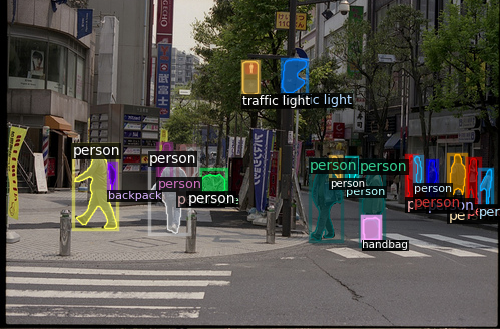
\includegraphics[width=\linewidth]{vis/success/val_848_det.png}
\end{minipage}
\begin{minipage}[b]{.24\linewidth}
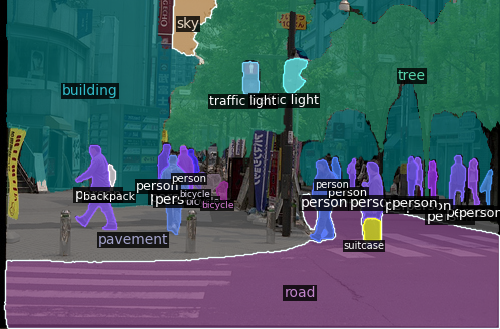
\includegraphics[width=\linewidth]{vis/success/val_848_pan.png}
\end{minipage}
\begin{minipage}[b]{.24\linewidth}
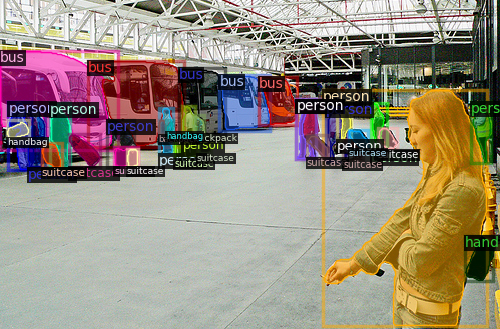
\includegraphics[width=\linewidth]{vis/success/val_965_det.png}
\end{minipage}
\begin{minipage}[b]{.24\linewidth}
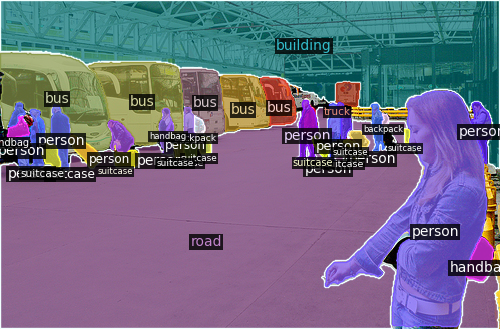
\includegraphics[width=\linewidth]{vis/success/val_965_pan.png}
\end{minipage}

\end{minipage}

\caption{\textbf{Qualitative results} for object detection and panoptic segmentation on the COCO~\cite{lin2014mscoco} 2017 \val set generated by \ours. Note that \ours gives good predictions on \emph{small} objects.}
\label{fig:vis}
% \vspace{-0.2in}
\end{figure}
%%%%%%%%%%%%%%%%%%%%%%%%%%%%%%%%%%%%%%%%%%%%%%%%%%%%%%%%%%%%%%%%%%%%

\boldparagraph{State-of-the-art comparison and scaling behavior.}
We show in \cref{tab:det_main,tab:panoptic} that \ours indicates strong performance on object detection, instance segmentation and panoptic segmentation. To be specific, our plain detector combined with a ViT, pre-trained using MAE \cite{he2022mae} or BEiTv2 \cite{peng2022beitv2}, presents good scaling behavior. When moving to large and huge models, our method outperforms multi-scale counterparts including the recent end-to-end Mask2Former segmentation model \cite{cheng2022mask2former}. Despite involving more advanced attention blocks designs, \ie, shifted window attention in Swin \cite{liu2021swintransformer} and pooling attention in MViT \cite{fan2021mvit}, detectors with hierarchical backbones benefit less from larger backbones. \ours is better than the plain-backbone detector, ViTDet, across all backbones in terms of both accuracy and inference speed.
% The visualization of the \ours prediction can be seen in \cref{fig:vis} (more visualizations are provided in the supplementary).
    
    
    %%%%%%%%%%%%%%%%%%%%%%%%%%%%%%%%%%%%%%%%%%%%%%%%%%%%%%%%%%%%%%%%%%%
    \begin{table}[t]
    \centering
    \footnotesize
    {
    {
    \tablestyle{2.75pt}{1.2}
    \begin{tabular}{lccccccccccc}
    \multicolumn{1}{l|}{\multirow{2}{*}{method}} & \multicolumn{1}{c}{\multirow{2}{*}{backbone}} & \multicolumn{1}{c|}{\multirow{2}{*}{pre-train}} & \multicolumn{4}{c|}{Object Detection} & \multicolumn{4}{c|}{Instance Segmentation} & \multirow{2}{*}{FPS} \\
    \multicolumn{1}{l|}{} & \multicolumn{1}{c}{} & \multicolumn{1}{c|}{} & AP$^\text{b}$ & AP$^\text{b}_\text{S}$ & AP$^\text{b}_\text{M}$ & \multicolumn{1}{c|}{AP$^\text{b}_\text{L}$} & $\text{AP}^\text{m}$ & $\text{AP}^\text{m}_\text{S}$ & $\text{AP}^\text{m}_\text{M}$ & \multicolumn{1}{c|}{$\text{AP}^\text{m}_\text{L}$} &  \\
    % \shline
    % \rowcolor{orange!30} \multicolumn{12}{l}{\footnotesize \textbf{Base models}} \\
    % \multicolumn{1}{l|}{{\color{mygray} Swin~\cite{liu2021swintransformer}}} & {\color{mygray} Swin-B} & \multicolumn{1}{c|}{\color{mygray} sup-22K} & {\color{mygray} 54.0} & {\color{mygray} -} & {\color{mygray} -} & \multicolumn{1}{c|}{{\color{mygray} -}} & {\color{mygray} 46.5} & {\color{mygray} -} & {\color{mygray} -} & \multicolumn{1}{c|}{{\color{mygray} -}} & {\color{mygray} 13} \\
    % \multicolumn{1}{l|}{Mask2Former~\cite{cheng2022mask2former}} & {Swin-B} & \multicolumn{1}{c|}{sup-22K} & \multicolumn{4}{c|}{\small n/a} & \textbf{48.1} & \textbf{27.8} & 52.0 & \multicolumn{1}{c|}{\textbf{71.1}} & {\small -} \\
    % \multicolumn{1}{l|}{{\color{mygray} MViT~\cite{fan2021mvit}}} & {\color{mygray} MViT-B} & \multicolumn{1}{c|}{\color{mygray} sup-22K} & {\color{mygray} 55.6} & {\color{mygray} -} & {\color{mygray} -} & \multicolumn{1}{c|}{{\color{mygray} -}} & {\color{mygray} \textbf{48.1}} & {\color{mygray} -} & {\color{mygray} -} & \multicolumn{1}{c|}{{\color{mygray} -}} & {\color{mygray} 11} \\
    % \multicolumn{1}{l|}{BoxeR~\cite{nguyen2022boxer}} & ViT-B & \multicolumn{1}{c|}{MAE} & 55.4 & - & - & \multicolumn{1}{c|}{-} & 47.7 & - & - & \multicolumn{1}{c|}{-} & 12 \\
    % \multicolumn{1}{l|}{{\color{mygray} ViTDet~\cite{li2022vitdet}}} & {\color{mygray} ViT-B} & \multicolumn{1}{c|}{\color{mygray} MAE} & {\color{mygray} 54.0} & {\color{mygray} 36.5} & {\color{mygray} 57.8} & \multicolumn{1}{c|}{{\color{mygray} 69.1}} & {\color{mygray} 46.7} & {\color{mygray} 27.2} & {\color{mygray} 49.6} & \multicolumn{1}{c|}{{\color{mygray} 64.9}} & {\color{mygray} 11} \\
    % % ************************************
    % \hline
    % \multicolumn{1}{l|}{{\color{mygray} UViT~\cite{chen2022uvit}}} & {\color{mygray} UViT-B} & \multicolumn{1}{c|}{\color{mygray} self-learning} & {\color{mygray} 53.9} & {\color{mygray} -} & {\color{mygray} -} & \multicolumn{1}{c|}{{\color{mygray} -}} & {\color{mygray} 46.1} & {\color{mygray} -} & {\color{mygray} -} & \multicolumn{1}{c|}{{\color{mygray} -}} & {\color{mygray} 12} \\
    % \multicolumn{1}{l|}{{PlainDETR~\cite{lin2023plaindetr}}} & {ViT-B} & \multicolumn{1}{c|}{MAE} & {53.8} & {35.9} & {57.0} & \multicolumn{1}{c|}{{68.9}} & \multicolumn{4}{c|}{\small n/a} & {12} \\
    % \multicolumn{1}{l|}{\ours} & {ViT-B} & \multicolumn{1}{c|}{MAE} & 55.6 & \textbf{37.1} & 59.2 & \multicolumn{1}{c|}{71.5} & 48.0 & {27.5} & 51.5 & \multicolumn{1}{c|}{67.8} & \textbf{15} \\
    % \multicolumn{1}{l|}{\ours} & {ViT-B} & \multicolumn{1}{c|}{BEiTv2} & \textbf{55.7} & {36.5} & \textbf{60.2} & \multicolumn{1}{c|}{\textbf{72.3}} & \textbf{48.1} & {26.7} & \textbf{52.7} & \multicolumn{1}{c|}{{68.9}} & \textbf{15} \\
    % % ************************************
    \shline
    \rowcolor{orange!50} \multicolumn{12}{l}{\footnotesize \textbf{Feature pyramids}} \\
    % \multicolumn{1}{l|}{{\color{mygray} Swin~\cite{liu2021swintransformer}}} & {\color{mygray} Swin-L} & \multicolumn{1}{c|}{\color{mygray} sup-22K} & {\color{mygray} 54.8} & {\color{mygray} -} & {\color{mygray} -} & \multicolumn{1}{c|}{{\color{mygray} -}} & {\color{mygray} 47.3} & {\color{mygray} -} & {\color{mygray} -} & \multicolumn{1}{c|}{{\color{mygray} -}} & {\color{mygray} \textbf{10}} \\
    % \multicolumn{1}{l|}{Mask2Former~\cite{cheng2022mask2former}} & {Swin-L} & \multicolumn{1}{c|}{sup-22K} & \multicolumn{4}{c|}{\small n/a} & 50.1 & 29.9 & 53.9 & \multicolumn{1}{c|}{\textbf{72.1}} & 4 \\
    % \multicolumn{1}{l|}{{\color{mygray} MViT~\cite{fan2021mvit}}} & {\color{mygray} MViT-L} & \multicolumn{1}{c|}{\color{mygray} sup-22K} & {\color{mygray} 55.7} & {\color{mygray} -} & {\color{mygray} -} & \multicolumn{1}{c|}{{\color{mygray} -}} & {\color{mygray} 48.3} & {\color{mygray} -} & {\color{mygray} -} & \multicolumn{1}{c|}{{\color{mygray} -}} & {\color{mygray} 6} \\
    % \multicolumn{1}{l|}{{\color{mygray} ViTDet~\cite{li2022vitdet}}} & {\color{mygray} ViT-L} & \multicolumn{1}{c|}{\color{mygray} MAE} & {\color{mygray} 57.6} & {\color{mygray} 40.5} & {\color{mygray} 61.6} & \multicolumn{1}{c|}{{\color{mygray} 72.6}} & {\color{mygray} 49.9} & {\color{mygray} 30.5} & {\color{mygray} 53.3} & \multicolumn{1}{c|}{{\color{mygray} 68.0}} & {\color{mygray} 7} \\
    \multicolumn{1}{l|}{{Swin~\cite{liu2021swintransformer}}} & {Swin-L} & \multicolumn{1}{c|}{sup-21K} & {55.0} & {38.3} & {59.4} & \multicolumn{1}{c|}{{71.6}} & {47.2} & {28.7} & {50.5} & \multicolumn{1}{c|}{{66.0}} & {10} \\
    \multicolumn{1}{l|}{Mask2Former~\cite{cheng2022mask2former}} & {Swin-L} & \multicolumn{1}{c|}{sup-21K} & \multicolumn{4}{c|}{\small n/a} & 50.1 & 29.9 & 53.9 & \multicolumn{1}{c|}{\textbf{72.1}} & 4 \\
    \multicolumn{1}{l|}{{MViT~\cite{fan2021mvit}}} & {MViT-L} & \multicolumn{1}{c|}{sup-21K} & {55.7} & {40.3} & {59.6} & \multicolumn{1}{c|}{{71.4}} & {48.3} & {31.1} & {51.2} & \multicolumn{1}{c|}{{66.3}} & {6} \\
    \multicolumn{1}{l|}{{ViTDet~\cite{li2022vitdet}}} & {ViT-L} & \multicolumn{1}{c|}{MAE} & {57.6} & {40.5} & {61.6} & \multicolumn{1}{c|}{{72.6}} & {49.9} & {30.5} & {53.3} & \multicolumn{1}{c|}{{68.0}} & {7} \\
    % ************************************
    \hline
    % \multicolumn{1}{l|}{{\color{mygray} MViT~\cite{li2022vitdet}}} & {\color{mygray} MViT-H} & \multicolumn{1}{c|}{\color{mygray} sup-22K} & {\color{mygray} 55.7} & {\color{mygray} -} & {\color{mygray} -} & \multicolumn{1}{c|}{{\color{mygray} -}} & {\color{mygray} 48.3} & {\color{mygray} -} & {\color{mygray} -} & \multicolumn{1}{c|}{{\color{mygray} -}} & {\color{mygray} 6} \\
    % \multicolumn{1}{l|}{{\color{mygray} ViTDet~\cite{li2022vitdet}}} & {\color{mygray} ViT-H} & \multicolumn{1}{c|}{\color{mygray} MAE} & {\color{mygray} 58.7} & {\color{mygray} 41.9} & {\color{mygray} 63.0} & \multicolumn{1}{c|}{{\color{mygray} 73.9}} & {\color{mygray} 50.9} & {\color{mygray} 32.0} & {\color{mygray} 54.3} & \multicolumn{1}{c|}{{\color{mygray} 68.9}} & {\color{mygray} 5} \\
    \multicolumn{1}{l|}{{MViT~\cite{li2022vitdet}}} & {MViT-H} & \multicolumn{1}{c|}{sup-21K} & {55.9} & {40.8} & {59.8} & \multicolumn{1}{c|}{{70.8}} & {48.3} & {30.1} & {51.1} & \multicolumn{1}{c|}{{66.6}} & {6} \\
    \multicolumn{1}{l|}{{ViTDet~\cite{li2022vitdet}}} & {ViT-H} & \multicolumn{1}{c|}{MAE} & {58.7} & {41.9} & {63.0} & \multicolumn{1}{c|}{{73.9}} & {50.9} & {32.0} & {54.3} & \multicolumn{1}{c|}{{68.9}} & {5} \\
    % ************************************
    \shline
    \rowcolor{orange!50} \multicolumn{12}{l}{\footnotesize \textbf{Plain features}} \\
    \multicolumn{1}{l|}{\ours} & {ViT-L} & \multicolumn{1}{c|}{MAE} & {58.5} & {42.2} & {62.5} & \multicolumn{1}{c|}{{73.4}} & 50.6 & {32.1} & {54.2} & \multicolumn{1}{c|}{69.8} & 9 \\
    \multicolumn{1}{l|}{\ours} & {ViT-L} & \multicolumn{1}{c|}{BEiTv2} & {58.7} & {40.4} & {63.2} & \multicolumn{1}{c|}{{74.8}} & {50.9} & {30.4} & {55.1} & \multicolumn{1}{c|}{70.9} & 9 \\
    % ------------------------------------------------------------------------------------------------
    \hline
    \multicolumn{1}{l|}{\ours} & {ViT-H} & \multicolumn{1}{c|}{MAE} & \textbf{59.8} & \textbf{42.2} & \textbf{63.8} & \multicolumn{1}{c|}{\textbf{74.9}} & \textbf{51.9} & \textbf{32.2} & \textbf{55.7} & \multicolumn{1}{c|}{{71.0}} & 7 \\
    \end{tabular}
    }
    }
    % \vspace{1em}
    \caption{\textbf{State-of-the-art comparison and scaling behavior for object detection and instance segmentation.} We compare methods using feature pyramids \vs plain features on COCO \val (n/a: entry is not available). Backbones with MAE pre-trained on ImageNet-1K while others pre-trained on ImageNet-21K. 
    % \ours indicates good scaling behavior. 
    With only single-scale features, \ours shows strong performance compared to multi-scale detectors including transformer-based detectors like Mask2Former, while being $\sim2\times$ faster.}
    \label{tab:det_main}
    % \vspace{-0.2in}
    \end{table}
    %%%%%%%%%%%%%%%%%%%%%%%%%%%%%%%%%%%%%%%%%%%%%%%%%%%%%%%%%%%%%%%%%%%%

    \begin{table}[t]
        \centering
        \footnotesize
        {
        \tablestyle{3.25pt}{1.2}
        \begin{tabular}{lcccccc}
        \multicolumn{1}{l|}{\multirow{2}{*}{method}} & \multirow{2}{*}{backbone} & \multicolumn{1}{c|}{\multirow{2}{*}{pre-train}} & \multicolumn{3}{c|}{Panoptic Segmentation} & \multirow{2}{*}{FPS} \\
        \multicolumn{1}{l|}{} &  & \multicolumn{1}{c|}{} & PQ & PQ$^\text{th}$ & \multicolumn{1}{c|}{PQ$^\text{st}$} & \\
        \shline
        \rowcolor{orange!50} \multicolumn{7}{l}{\footnotesize \textbf{Feature pyramids}} \\
        \multicolumn{1}{l|}{MaskFormer~\cite{cheng2021maskformer}} & Swin-B & \multicolumn{1}{c|}{sup-21K} & 51.8 & 56.9 & \multicolumn{1}{c|}{44.1} & - \\
        \multicolumn{1}{l|}{Mask2Former~\cite{cheng2022mask2former}} & Swin-B & \multicolumn{1}{c|}{sup-21K} & 56.4 & 62.4 & \multicolumn{1}{c|}{47.3} & - \\
        \hline
        \multicolumn{1}{l|}{Mask2Former~\cite{cheng2022mask2former}} & Swin-L & \multicolumn{1}{c|}{sup-21K} & 57.8 & 64.2 & \multicolumn{1}{c|}{48.1} & 4 \\
        \shline
        \rowcolor{orange!50} \multicolumn{7}{l}{\footnotesize \textbf{Plain features}} \\
        \multicolumn{1}{l|}{\ours} & ViT-B & \multicolumn{1}{c|}{BEiTv2} & {56.5} & {62.6} & \multicolumn{1}{c|}{{47.3}} & {13} \\
        \hline
        \multicolumn{1}{l|}{\ours} & ViT-L & \multicolumn{1}{c|}{BEiTv2} & \textbf{58.5} & \textbf{65.1} & \multicolumn{1}{c|}{\textbf{48.6}} & {8} \\
        \end{tabular}
        }
        % \vspace{1em}
        {\caption{\textbf{State-of-the-art comparison and scaling behavior for panoptic segmentation.} We compare between methods using feature pyramids (\emph{top} row) \vs single-scale (\emph{bottom} row) on COCO~\val. \ours with single-scale input shows better results when scaling to larger backbones, while being $\sim2\times$ faster compared to Mask2Former.}\label{tab:panoptic}}%
    \end{table}

    \boldparagraph{Limitations.} Our final goal is to simplify the detection pipeline and to achieve competitive results at the same time. In \cref{sec:experiments}, we find that the \emph{adaptive-scale} attention mechanism that adaptively learns scale-aware information in its computation plays a key role for a plain detector. However, our adaptive-scale attention still encodes the knowledge of different scales. In the future, we hope that with the large-scale training data, a simpler design of the attention mechanism could also learn the scale equivariant property. Furthermore, \ours faces difficulties in detecting and segmenting large objects in the image. To overcome this limitation, we think that a design of attention computation which effectively combines both global and local information is necessary.


\section{Conclusion}
\label{sec:conclusion}

We presented \ours, a simple and plain object detector that eliminates the requirement for handcrafting multi-scale feature maps. Through our experiments, we demonstrated that a transformer-based detector, equipped with a scale-aware attention mechanism, can effectively learn scale-equivariant features through data. The efficient design of \ours allows it to take advantages of significant progress in scaling ViTs, reaching highly competitive performance on three tasks on COCO: object detection, instance segmentation, and panoptic segmentation. This finding suggests that many handcrafted designs for convolution neural network in computer vision could be removed when moving to transformer-based architecture. We hope this study could encourage future exploration in simplifying neural network architectures especially for dense vision tasks.


% ---- Bibliography ----
%
% BibTeX users should specify bibliography style 'splncs04'.
% References will then be sorted and formatted in the correct style.
%
{
  \small
  \bibliographystyle{splncs04}
  \bibliography{simplr}
}
\end{document}
